
\section{Case study Example}\label{sec:metriccase}
In this section the centrality metrics discussed in \autoref{sec:graphcentrality} are applied to a range of senarios. These range from polluted urban environments such as London [REF] and Beijing [REF], to marine and terrestial forrest- Cape Verde REF and Borneo REF. We determine the main drivers for the chemistry and compare the species which are important across each simulation.  

\subsection{Establishing Initial Conditions from observational data}
Within experimental data assimulation it is not uncommon to face problems which resut in unreliable or missing data. These can range from anything as little as measuring below the instrument sensitivity to powercuts and equiptment damage/theft from the local wildlife. This can result in problems when analysing the results and combining them to create a simulation of the chemistry for that environment. 

To overcome this, traditionally a combination of data filtration, smoothing and interpolation is required. Although it is possible to fit a diurnal profile, through itereative methods of comparison, and cubic splines, a much simpler way would be to use an Multi Layer Perceptron Regressor model (MLPRegressor) as provided by sklearn, \citep{sklearn}. This is described below.

\subsubsection{The origin of Artificial Neural Networks}
The concept of a neural network originated witin the field of neuroscience. In in bilogical neurons, signals are sent through the use of electrical impulses using their synapses. When a sufficient number of signals are recieved within a short timeframe, a neurone will respond, often firing a range of its own signals. Using this as a foundation,\cite{pitts} presented a computational model of the biological neuron - the artifical neuron. This has a series of binary inputs, and produces a single binary output. This idea was later imporoved with the invention of the perceptron - a linear classifier which classifies categories by separating them with a straight line. Invented by \cite{perceptron}, this was popularised as a device representative of a modern day shallow neural network - \citep{perceptronmanual}, \autoref{fig:perceptron}. Unlike the artificial neuron however, the perceptron is able to take non-binary (numerical) inputs of an associated weight which allows for the computation of simple linear binary classification. Much like Logistic regression, the preceptron produces a positive or negative classification based on a certain threshold\footnote{It is worth noting that while a Logistic Regression classifier can output a class probability, the use of a hard threshold means that this is not done within the preceptron algorithm \citep{handsonml}}. 


\begin{figure}[H]
     \centering
         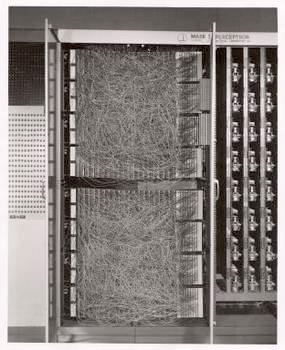
\includegraphics[width=.45\textwidth]{figures_c3/mlpregressor/Mark_I_perceptron.jpg}
        \caption{\textbf{The Mark 1 perceptron} Both software and hardware are different manifestations of a flow chart. The perceptron hardware accomplished what is now done using software. Source: \cite{perceptronimage}}
        \label{fig:perceptron}
\end{figure}

\subsubsection{The Multi Layer Perceptron}
Limitations of ther perceptron include the classifiction of complex patterns such as the XOR problem (where a category appears between two other categories e.g. {1|0|1} - this cannot be classified by a single linear split). In taking inspiration from nature, \autoref{fig:layercortex}, it is possible to overcome this with the use of multiple layers. This creates an a deep ($>2$ two hidden (non-input) layers of perceptrons\footnote{These are sometimes refered as Linear Threshold Units.}) artificial neural network (ANN) 

The multi layer perceptron (MLP) model now represents a simple feed-forwards network, much like a decision tree. However unlike a decision tree, the MLP ANN is able to describe the probability a branch is taken using non-linear activation (threshold) functions. These are discussed in detail as part of SECTION NEXT CHAPTER. The weighting thresholds for each neuron are then calculated by backwards propagation of results through the network until a suitably good result is produced. 

\begin{quote}
\textit{
\textbf{Example analogy:} Back propagation can be likened to the iterative calibration of scientific instrumentation. In the field of atmopsheric chemistry laser induced flourecence is used to calculate species concentrations and reaction rates within the troposphere, \citep{lif1,lif2}. Here the frequency of a laser can be adjusted in contrast with a known target (e.g. an amount of \ce{SO2}) to produce a responce curve showing where the maximum resonance occurs.\\
Similarly a neural network can be `trained' (calibrated). 
This is done through the use of a `training dataset' - a set of input-output pairings which represent a random selectaion of 2/3rds of the total dataset. Next the neurons within each layer (similar to the potentiometer dials on an instrument) are adjusted in sequence through the layers to match the known result (a standard of known concentration) to the input values provided. This process is repeated until for a number of iterations, or until a sufficently `good' prediction is attained for the entire training dataset (early termination). The power of ANNs comes from the ability to adjust neuron thresholds whilst moving both forwards and backwards through the network (Note: predictions of a MLP are still only passed forwards). Finally model perfomance is evaluated against the remaining 1/3rd of the total dataset.
}
\end{quote}


\begin{figure}[H]
     \centering
         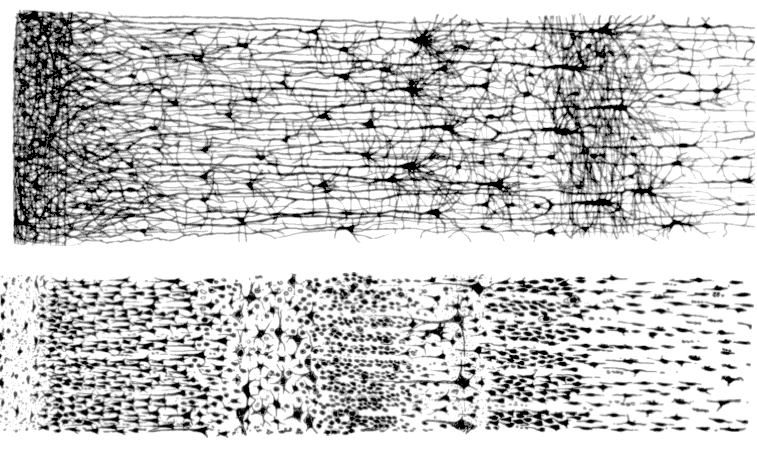
\includegraphics[width=.85\textwidth]{figures_c3/mlpregressor/Cajal_cortex_drawings.png}
        \caption{\textbf{The Human Cortex - A biological neural network.}. A vertical cross section of the human cortex between an adult (top) and 1.5 month old infant (bottom) showing a layer like structure with a change in depth (left to right). Source: \cite{layercortex}}
        \label{fig:layercortex}
\end{figure}

\subsubsection{Application of the MLPRegressor to observational data}
In the application of any type of machine aided algorithms it is important to evaluate the results provided. In this section the results of 12 years of data collected as part of the [CAPE VERDE CAMPAIGN] are shown (these contain measurements spanning the entirety of 12 years, which produce the clearest tests for the algorithm). A MLPRegressor of 10 hidden layers, and a hyperbolic tan (tanh) activation function is used. Additionally the limited-memory Broyden–Fletcher–Goldfarb–Shanno (l-BFGS) solver (a quasi-newton method which minimises the inverse of the Hessian matrix\footnote{ The hessian is square matrix of second-order partial derivatives of a scalar-valued function/field describing the local curvature of a function (of many variables).} to steer through space and obtain a solution) and an adaptive learning rate\footnote{Each time the model improvement fails to decrease the learning loss, the learning rate is reduced by 1/5. This means smaller jumps are made towards the curve peak. } is used. 

Input of the regressor is in the from of a month and a hour, to represent each measurement. This allows it to find not only daily trends, but also seasonal trends within the data. Once trained the regressor is then used to predict a diurnal profile for each month based on the observational data provided. For simplicity $\log_{10}$ values of the concentrations obtained have been used. To validate the results, the predicted MLPRegressor line is compared to a transparent scatterplot for all the results. In addition to this a boxplot showing the IQR, median and mean (green line) plotted alongside to evaluate the predictor output. 

In providing the MLPRegressor with both month and hour inputs, the data is not only fitted hourly (a diurnal avarage), but also across the seasonal/monthly cycles. This accounts for the variation between years and datasets. Since $\log_{10}$ values of the concentrations are used, species such as ozone (\autoref{fig:mlpo3}) which for the Cape Verde dataset (clean air) do not change more than one order of magnitude, the effects of neigbouring months, which shift the diurnal away from the mean (the green line on the boxplot), can be seen. However since this is overall a small change, and the diurnals lie within the inter quartile range, they still provide an adequate approximation. NO (\autoref{fig:mlpno}) on the other hand has a concentration change of several orders of magnitude. Here a distinct daytime peak is seen and is centred around a sesonally consistent mean value of the data. Here the multi-magnitude change in concentration also provides an effective silhouette of the data to which we may compare the fitted line. 
Finally the plots of \ce{NO2} and iso-Pentane (\autoref{fig:mlpno2}-\ref{fig:mlpisopentane}) vary both in diurnal magnitude and seasonally. Within these plots, changes in the data in the january and december months produce deceptively misleading results. Here although the diurnals are not symmetrix, they fit well within the median,mean and interquartile range values, as well as the general data silhouette behind them. This siggests that it is a property of the data that we are fitting, and not that the regressor is producing incorrect results. It is however noted that for a more accurate seasonal prediction, periodic boundary conditions should be employed in the training dataset, where an additional two months are added before January and after December. 

Since I shall be using only a noon estimate from the summer region, this does not affect any of the results. 

\begin{figure}[H]
     \centering
         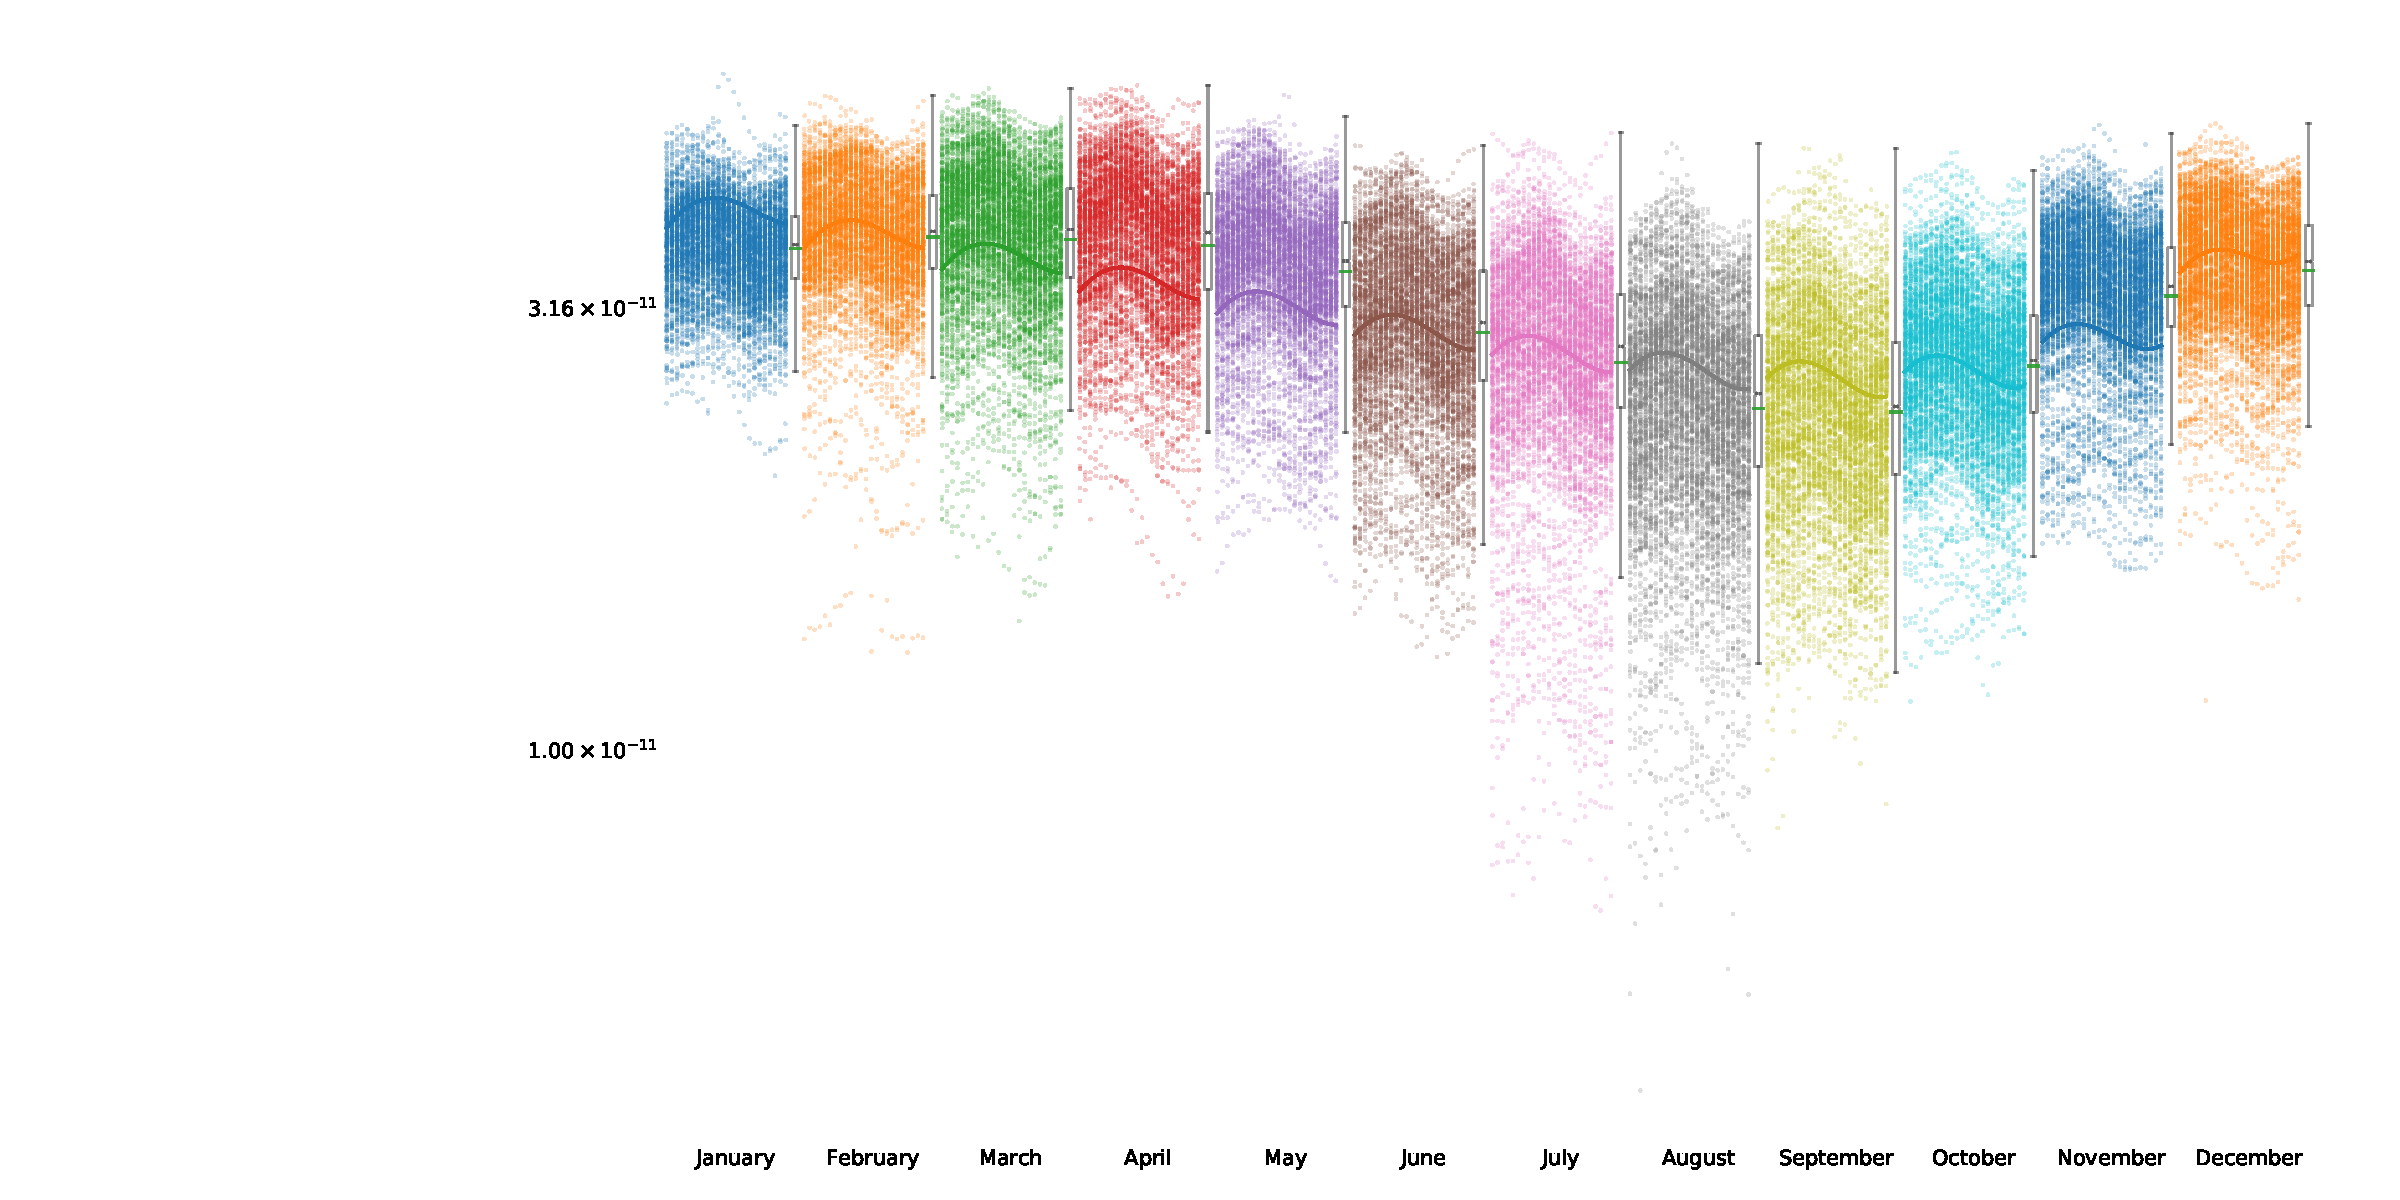
\includegraphics[width=.90\textheight,angle =90,trim={8cm 0 0 0}]{figures_c3/mlpregressor/CVNOX_CapeVerde/O3.pdf}
        \caption{\textbf{Cape Verde MLP predicted and observational data of Ozone.} Each segment represents data from a different month. Within each month segment exists 24 hour segments to create a diurnal. Observational concentrations are plotted in the form of a translucent scatterplot and summarised using the boxplot on the right of the month segment. MLP predicted results are shown using the solid lines. Concentration in mixing ratio.}
        \label{fig:mlpo3}
\end{figure}

\begin{figure}[H]
     \centering
         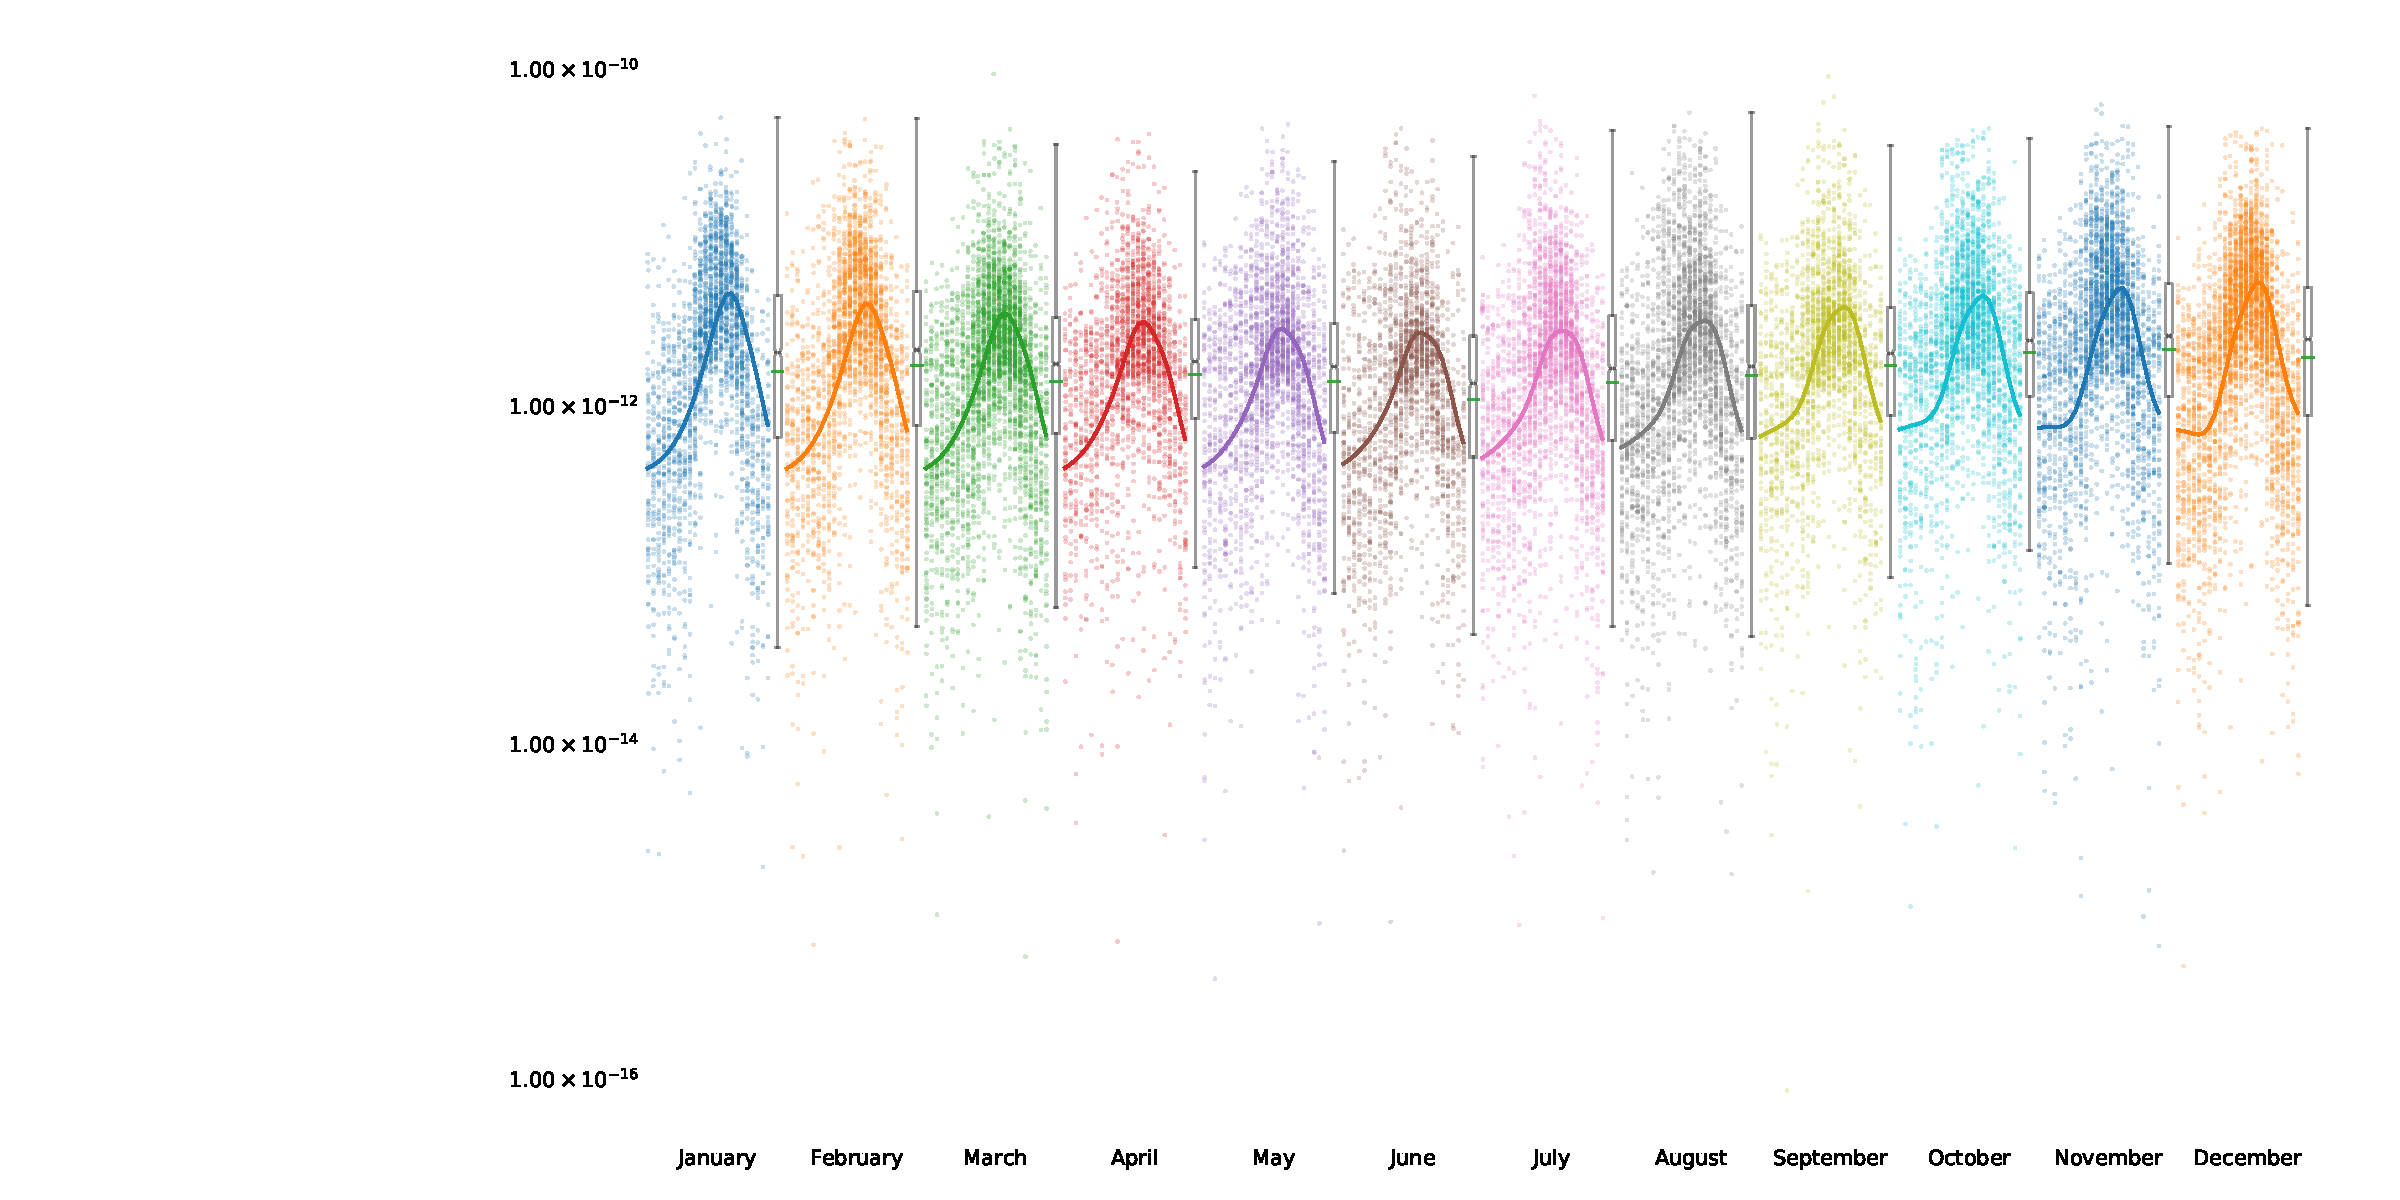
\includegraphics[width=.90\textheight,angle =90,trim={8cm 0 0 0}]{figures_c3/mlpregressor/CVNOX_CapeVerde/NO.pdf}
        \caption{\textbf{Cape Verde MLP predicted and observational data of NO.} Each segment represents data from a different month. Within each month segment exists 24 hour segments to create a diurnal. Observational concentrations are plotted in the form of a translucent scatterplot and summarised using the boxplot on the right of the month segment. MLP predicted results are shown using the solid lines. Concentration in mixing ratio.}
        \label{fig:mlpno}
\end{figure}

\begin{figure}[H]
     \centering
         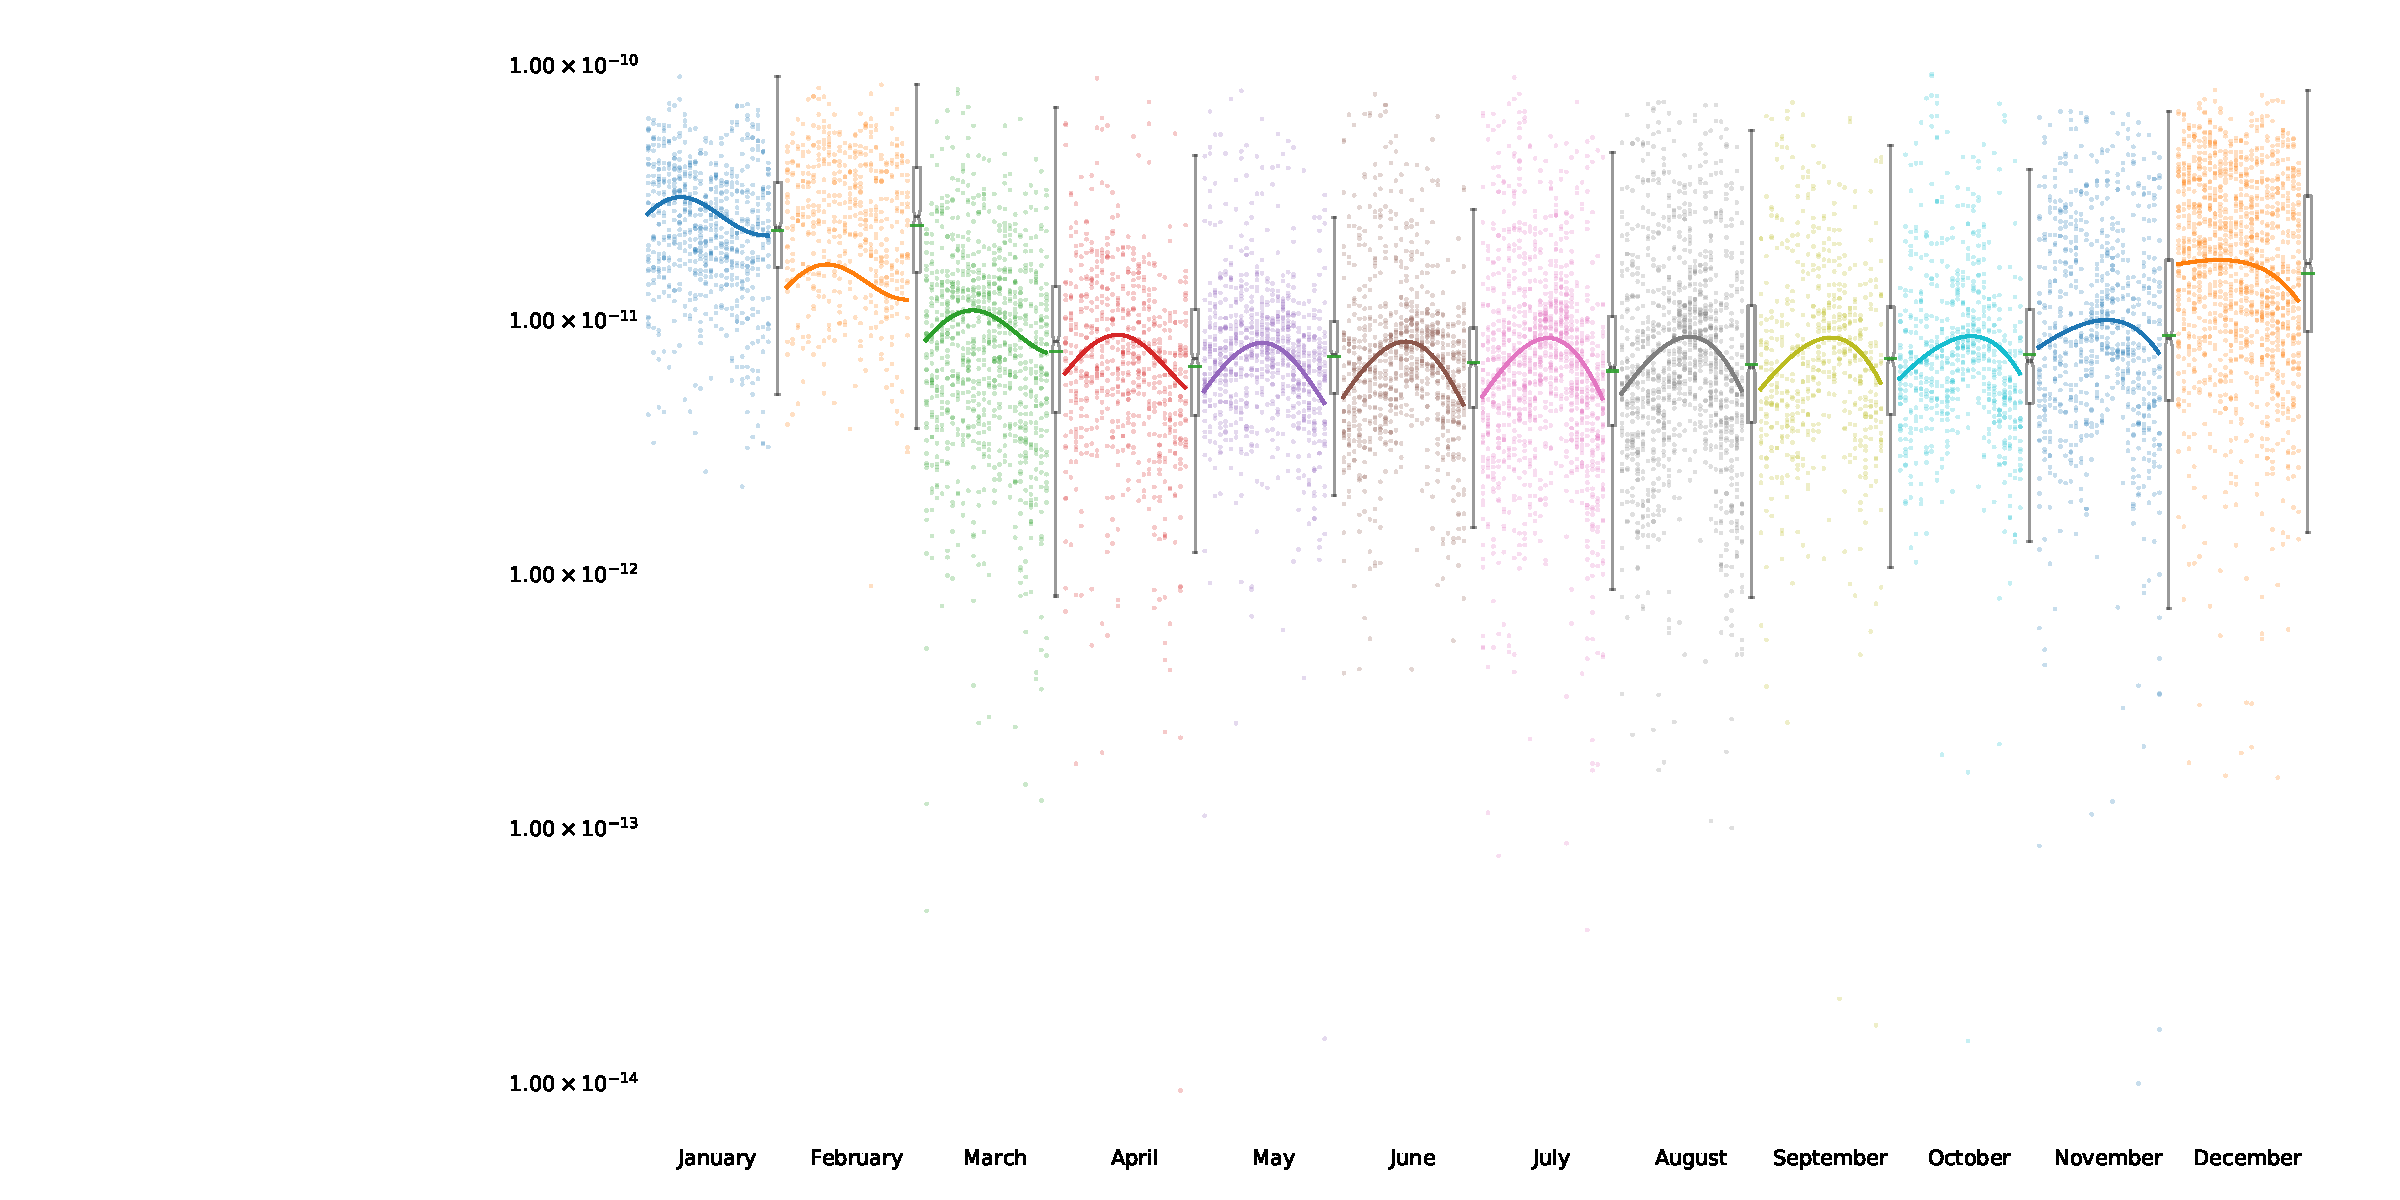
\includegraphics[width=.90\textheight,angle =90,trim={8cm 0 0 0}]{figures_c3/mlpregressor/CVNOX_CapeVerde/NO2.pdf}
        \caption{\textbf{Cape Verde MLP predicted and observational data of \ch{no2}.} Each segment represents data from a different month. Within each month segment exists 24 hour segments to create a diurnal. Observational concentrations are plotted in the form of a translucent scatterplot and summarised using the boxplot on the right of the month segment. MLP predicted results are shown using the solid lines. Concentration in mixing ratio.}
        \label{fig:mlpno2}
\end{figure}

\begin{figure}[H]
     \centering
         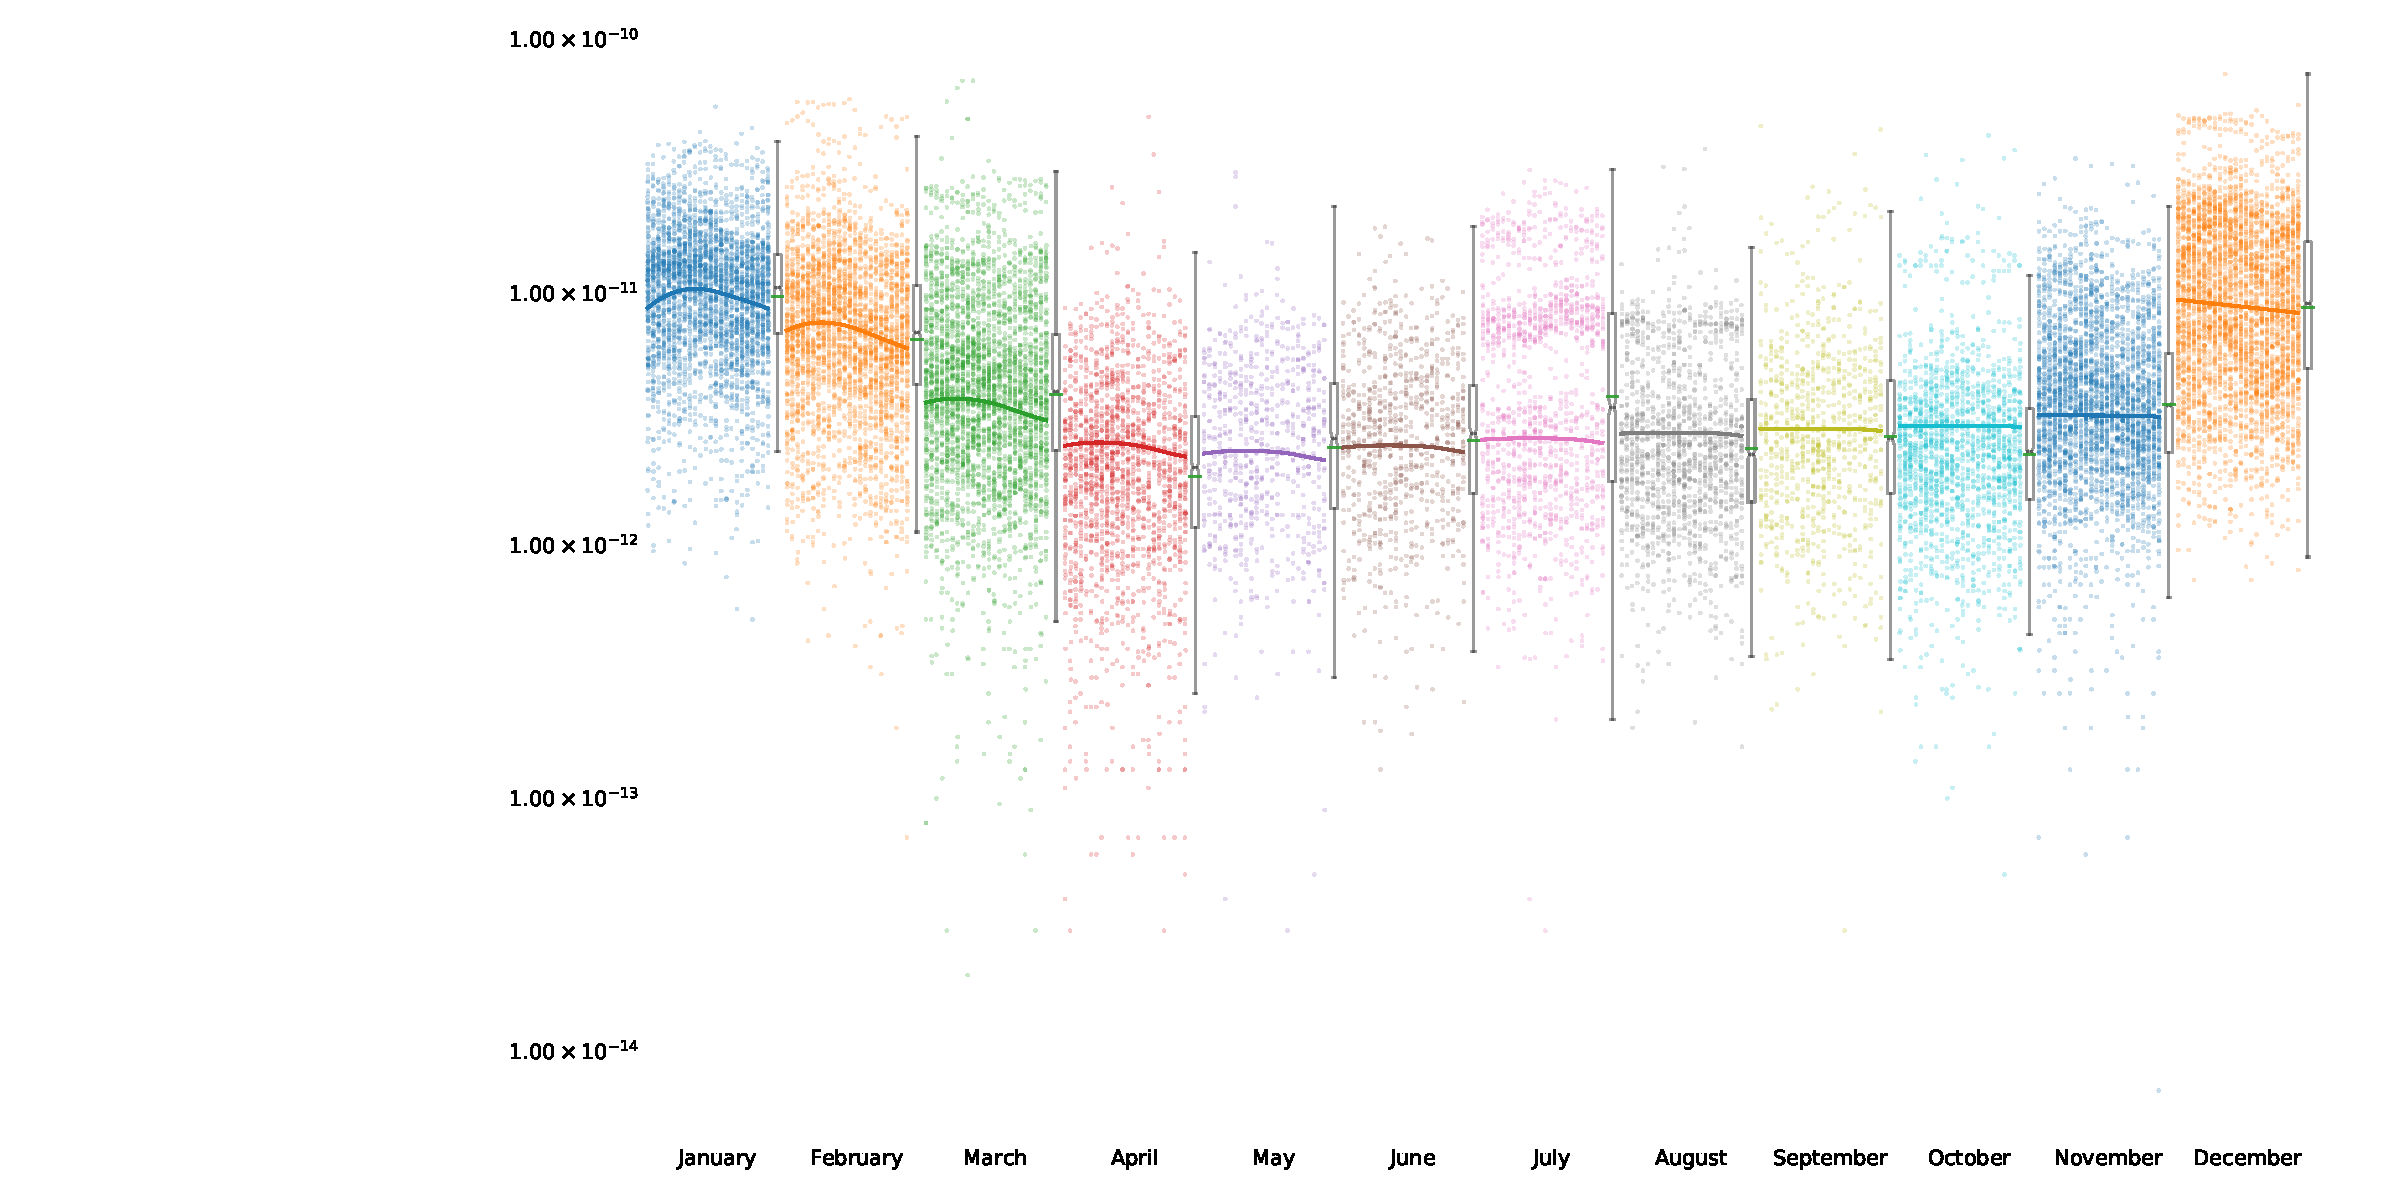
\includegraphics[width=.90\textheight,angle =90,trim={8cm 0 0 0}]{figures_c3/mlpregressor/CVNOX_CapeVerde/ISO_PENTANE.pdf}
        \caption{\textbf{Cape Verde MLP predicted and observational data of iso-Pentane.} Each segment represents data from a different month. Within each month segment exists 24 hour segments to create a diurnal. Observational concentrations are plotted in the form of a translucent scatterplot and summarised using the boxplot on the right of the month segment. MLP predicted results are shown using the solid lines. Concentration in mixing ratio. }
        \label{fig:mlpisopentane}
\end{figure}


\subsubsection{Generation of the ICS file and simulation run}

To generate the initial conditions for a model run, the MLP regressor is used to predict a representative species concentration at noon. As campaigns run at different times in the year, an error of $\pm 2 months$ around June exists. 

The predicted initial conditions in \autoref{tab:icsmetric} are used to initiate a box model simulation. 
To spin these up the initial concentrations are reset at noon each day. When the simulation reaches a fractional difference of less than 0.001, the model is left to run unconstrained for 5 days. Observation of the concentration profiles of each run (\autoref{fig:ccape}-\ref{fig:cbeijing}) show us how RO$_2$, HO$_x$, NO$_x$ and Ozone change over time. Within these it can be seen that RO$_2$ takes longer to stabilise in the polluted environments (London and Beijing) than those with cleaner air (Cape Verde and Borneo). Using the concentration profiles as a guide the instantaneous values for the simulation results are taken at noon, 3 days after the end of the spinup period. 

\subsubsection{Extracting the required results}
Model diagnostics such as concentration and the net flux passing through a species may be extracted directly from the DSMACC box model. These provide the baseline comparison against which we shall compare the results of graph metrics. The concentration will tell us which species are most abundant, and the net-flux tells us which are the fastest changing (either as a production or loss). 

In addition to this the jacobian matrix at the final timestep shall also be extracted. This is then manipulated to remove negative links (AS IN SECTION XX) and normalised. Using the normalised jacobian as an adjacency matrix, a graph on which the centrality metrics can be applied is generated. The result of these is compared in the next section.

\subsubsection{Unifying the results}
Since each metric compared can produce results on a different scale, there needs to be a method of normalising the results to achive parity between the range in which species are ranked. To do this all values within a group can be scaled between zero and unity, where 1 is the highest ranked and 0 is the lowest. For entries such as concentration or flux, which span several orders of magnitude, the $\log_{10}$ of the values shall be taken before they are scaled. 

\begin{table}[H]
    \centering
    \label{tab:icsmetric}
\begin{small}


\begin{table}[H]
\centering
\small

%%%%%%%
\begin{tabular}{p{0.2\textwidth}p{0.16\textwidth}p{0.16\textwidth}p{0.16\textwidth}p{0.16\textwidth}}
\toprule
Species & Beijing(APHH) & Borneo(OP3) &  London(ClearFlo) &  CapeVerde \\
\midrule
\ce{LAT}       & 39.9 &              0.96 &            51.0&       16.5 \\
\ce{LON}       &  116.3 &              114.5 &            0.00 &       23.4 \\
\midrule
CO & 3.829e-06 & 3.321e-07& 7.780e-09 & 0.0*\\
\ce{O3}        &  6.883e-08 &              8.939e-09 &            3.819e-08 &       2.629e-11* \\
\ce{NO}        &  1.660e-09 &              2.668e-14* &            2.350e-09 &       2.358e-12 \\
\ce{NO2}       &  1.226e-08 &              1.081e-13* &            7.445e-09 &       8.447e-12 \\
\ce{HCHO}      &  4.472e-09 &                        &            1.119e-08 &                 \\
\ce{C2H6}      &  3.163e-09 &              7.315e-10 &            2.133e-09 &       4.539e-10 \\
\ce{C2H4}      &  1.004e-09 &              1.152e-10 &            4.893e-10 &       2.481e-11 \\
\ce{C3H8}      &  3.019e-09 &              1.924e-10 &            1.128e-09 &       1.728e-11 \\
\ce{C3H6}      &  1.335e-10 &              1.333e-11 &            1.784e-10 &       9.343e-12 \\
\ce{IC4H10}    &  6.412e-10 &              8.742e-11 &            5.142e-10 &       2.486e-12 \\
\ce{NC4H10}    &  1.593e-09 &              5.698e-11 &            1.058e-09 &       4.481e-12 \\
\ce{C2H2}      &  1.058e-09 &              1.825e-10 &            3.018e-10 &       1.848e-11 \\
{TBUT2ENE}  &  4.198e-11 &                        &            1.815e-11 &                 \\
{CBUT2ENE}  &  4.454e-11 &                        &            1.305e-11 &                 \\
\ce{IC5H12}    &  1.047e-09 &              2.883e-11 &            7.424e-10 &       3.470e-12 \\
\ce{NC5H12}    &  4.650e-10 &              2.090e-11 &            2.792e-10 &       2.513e-12 \\
{TPENT2ENE} &  3.939e-11 &                        &                      &                 \\
{CPENT2ENE} &  3.982e-11 &                        &                      &                 \\
\ce{NC6H14}    &  2.057e-10 &              6.437e-12 &            6.357e-11 &                 \\
\ce{C5H8}      &  7.134e-10 &              1.957e-09 &            1.640e-10 &                 \\
\ce{NC7H16}    &  7.905e-11 &                        &            5.222e-11 &                 \\
\ce{BENZENE}   &  4.045e-10 &                        &            1.137e-10 &       7.682e-12 \\
\ce{NC8H18}    &  3.091e-11 &                        &            1.442e-11 &                 \\
\ce{TOLUENE}   &  6.767e-10 &                        &            3.205e-10 &       3.121e-12 \\
\ce{EBENZ}     &  3.115e-10 &                        &            6.017e-11 &                 \\
\ce{OXYL}      &  1.677e-10 &                        &            5.049e-11 &                 \\
\ce{CH3CHO}    &  4.783e-10 &                        &            4.095e-09 &                 \\
\ce{C2H5OH}    &  4.655e-09 &                        &            3.125e-09 &                 \\
\ce{CH3COCH3}  &  3.328e-09 &                        &            2.924e-09 &                 \\
\ce{NC9H20}    &  1.336e-11 &                        &            7.922e-11 &                 \\
\ce{NC10H22}   &  1.062e-12 &                        &            1.602e-10 &                 \\
$\alpha$-\ce{PINENE}\footnotemark
   &  7.341e-11 &     15e-11                   &            1.105e-10 &                 \\
\ce{LIMONENE}  &  5.836e-11 &              1.351e-10 &            3.566e-11 &                 \\
\ce{PXYL+MXYL}\footnotemark
 &  4.943e-10 &                        &                      &                 \\
\ce{IPBENZ}    &  4.567e-10 &                        &                      &                 \\
\ce{PBENZ}     &  3.996e-10 &                        &                      &                 \\
\ce{HONO}      &  6.479e-10 &                        &            4.109e-10 &                 \\
\ce{MACR}      &            &              6.948e-11 &            1.862e-11 &                 \\

%%%%%%%%%%%%%%%
\bottomrule
\end{tabular}
\end{table}


\begin{table}[H]
\centering
\small
\begin{tabular}{p{0.2\textwidth}p{0.16\textwidth}p{0.16\textwidth}p{0.16\textwidth}p{0.16\textwidth}}
\toprule
Species & Beijing(APHH) & Borneo(OP3) &  London(ClearFlo) &  CapeVerde \\
\midrule

%%%%%%%%%%%%%%

{PENT1ENE}  &            &                        &            2.383e-11 &                 \\
\ce{MVK}       &            &                        &            2.091e-11 &                 \\
\ce{NPROPOL}   &            &                        &            2.883e-10 &                 \\
\ce{NBUTOL}    &            &                        &            4.535e-10 &                 \\
\ce{STYRENE}   &            &                        &            2.241e-11 &                 \\
\ce{MEK}       &            &                        &            5.494e-11 &                 \\
\ce{C3H7CHO}   &            &                        &            9.534e-12 &                 \\
\ce{C4H9CHO}   &            &                        &            1.865e-11 &                 \\
\ce{C5H11CHO}  &            &                        &            1.201e-11 &                 \\
\ce{CYHEXONE}  &            &                        &            9.790e-12 &                 \\
\ce{BENZAL}    &            &                        &            1.510e-11 &                 \\
\ce{PAN}       &            &                        &            1.791e-10 &                 \\
\bottomrule
\end{tabular}


\caption{(2-page split) The initial conditions created from the MLPRegressor prediction of observational data. Although not specified the mixing ratios for methane is set by the model at 1770ppb, the temperature is 298K, and water vapour is at 2\%. \textbf{* Starred values are of the wrong units and should be multiplied by 1000. As there was no time to rerun these, their results have been omitted from this chapter.}}
\label{tab:icsmetric}
\end{table}

\footnotetext{This is (incorrectly) written as `?-pinene' in the merged CEDA dataset for the Borneo OP3 campaign. This is due to character conversion errors.}
\footnotetext{The mixing ratios for these is split evenly between both species}

\end{small}

\caption{The initial conditions created from the MLPRegressor prediction of observational data.}
\end{table}
\footnotetext{This is written as ?-pinene in the merged CEDA dataset for the Borneo OP3 campaign. This is due to character conversion errors.}
\footnotetext{The concentration for these is split evenly between both species}
\newpage


\begin{figure}[H]
    \centering
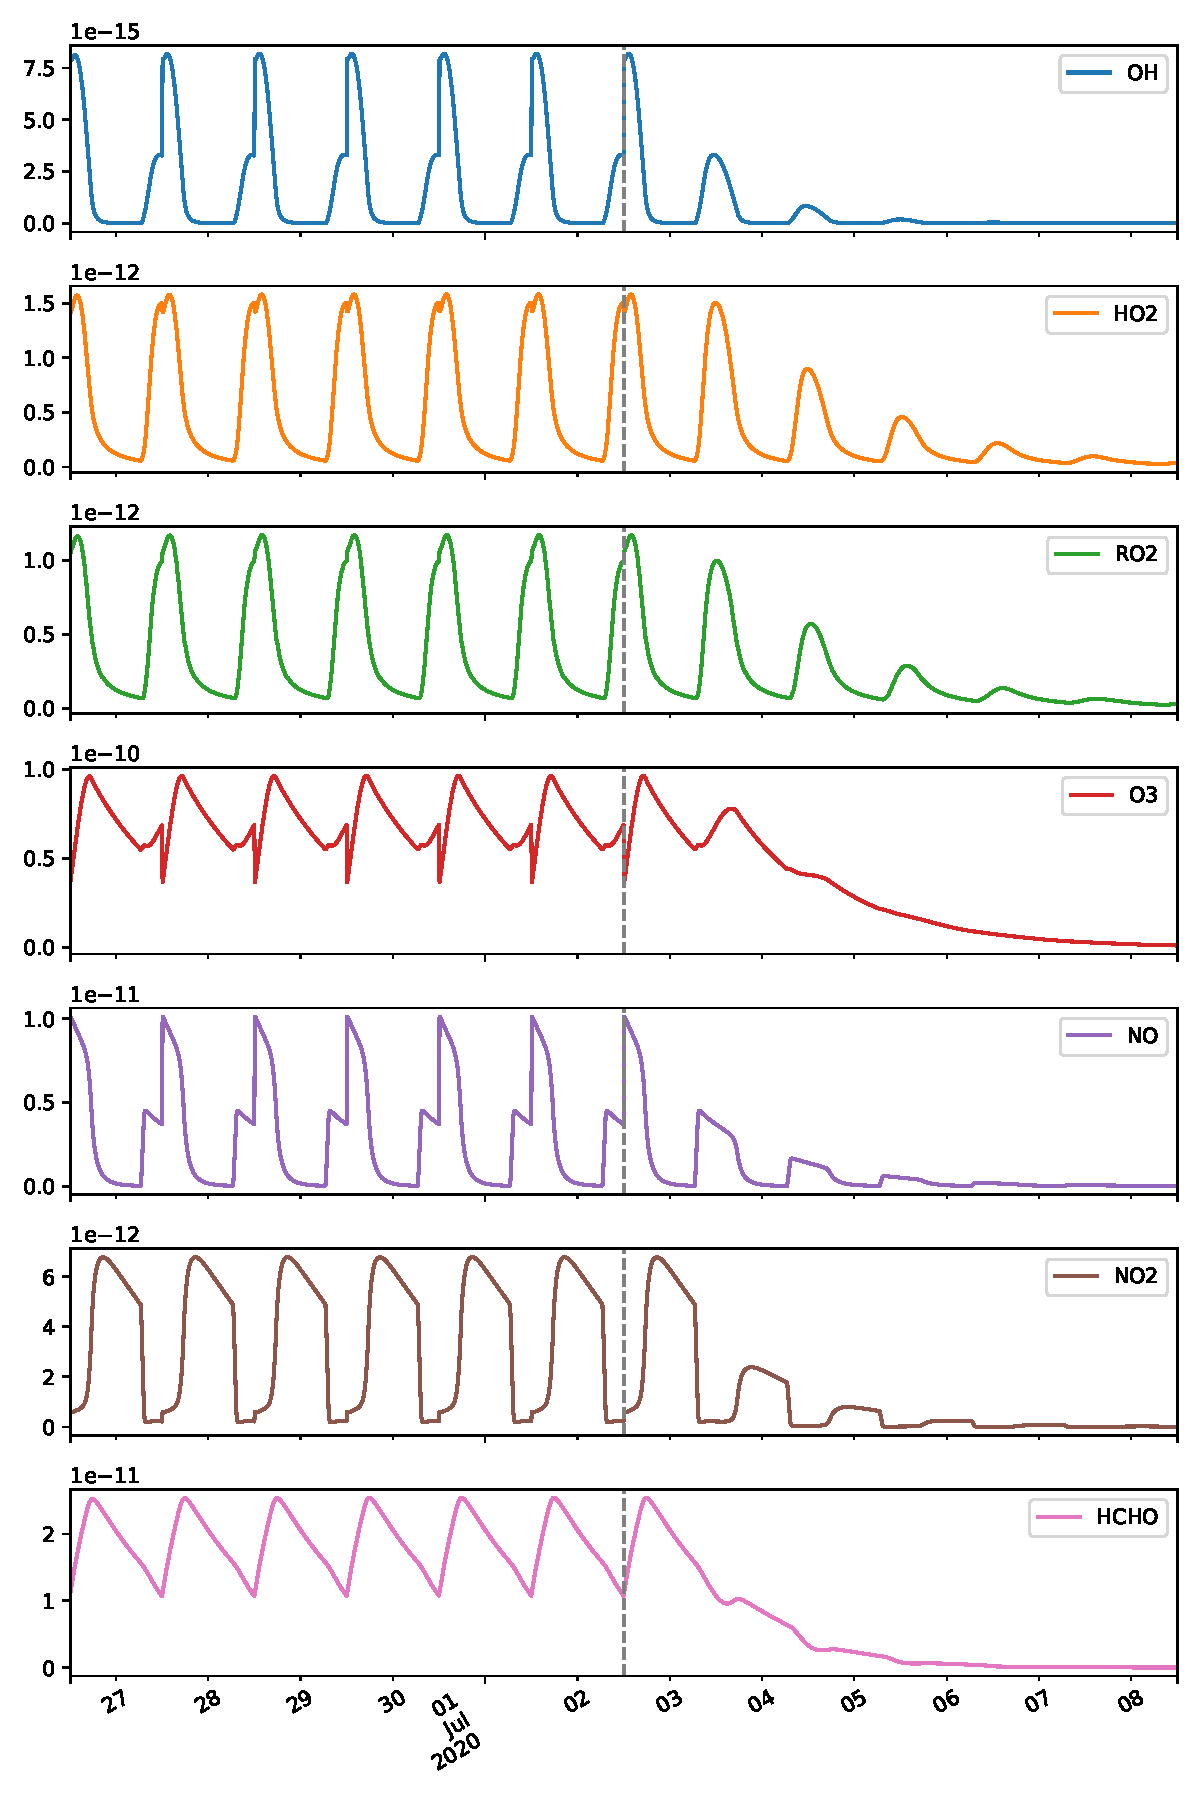
\includegraphics[width=.9\textwidth]{figures_c3/mlpregressor/conc_cape.pdf}
\label{fig:ccape}
\caption{\textbf{The concentration profile for CapeVerde.}This shows a the change in concentration over time for HO$_x$,NO$_x$,Ozone and RO$_2$ species for a simulation run generated by the mlpregressor. Left of the dashed line shows the last 6 days of spinup, where the intial concentrations are reset at noon each day until the species fractional difference is less than 0.001 .}
\end{figure}

\newpage


\begin{figure}[H]
    \centering
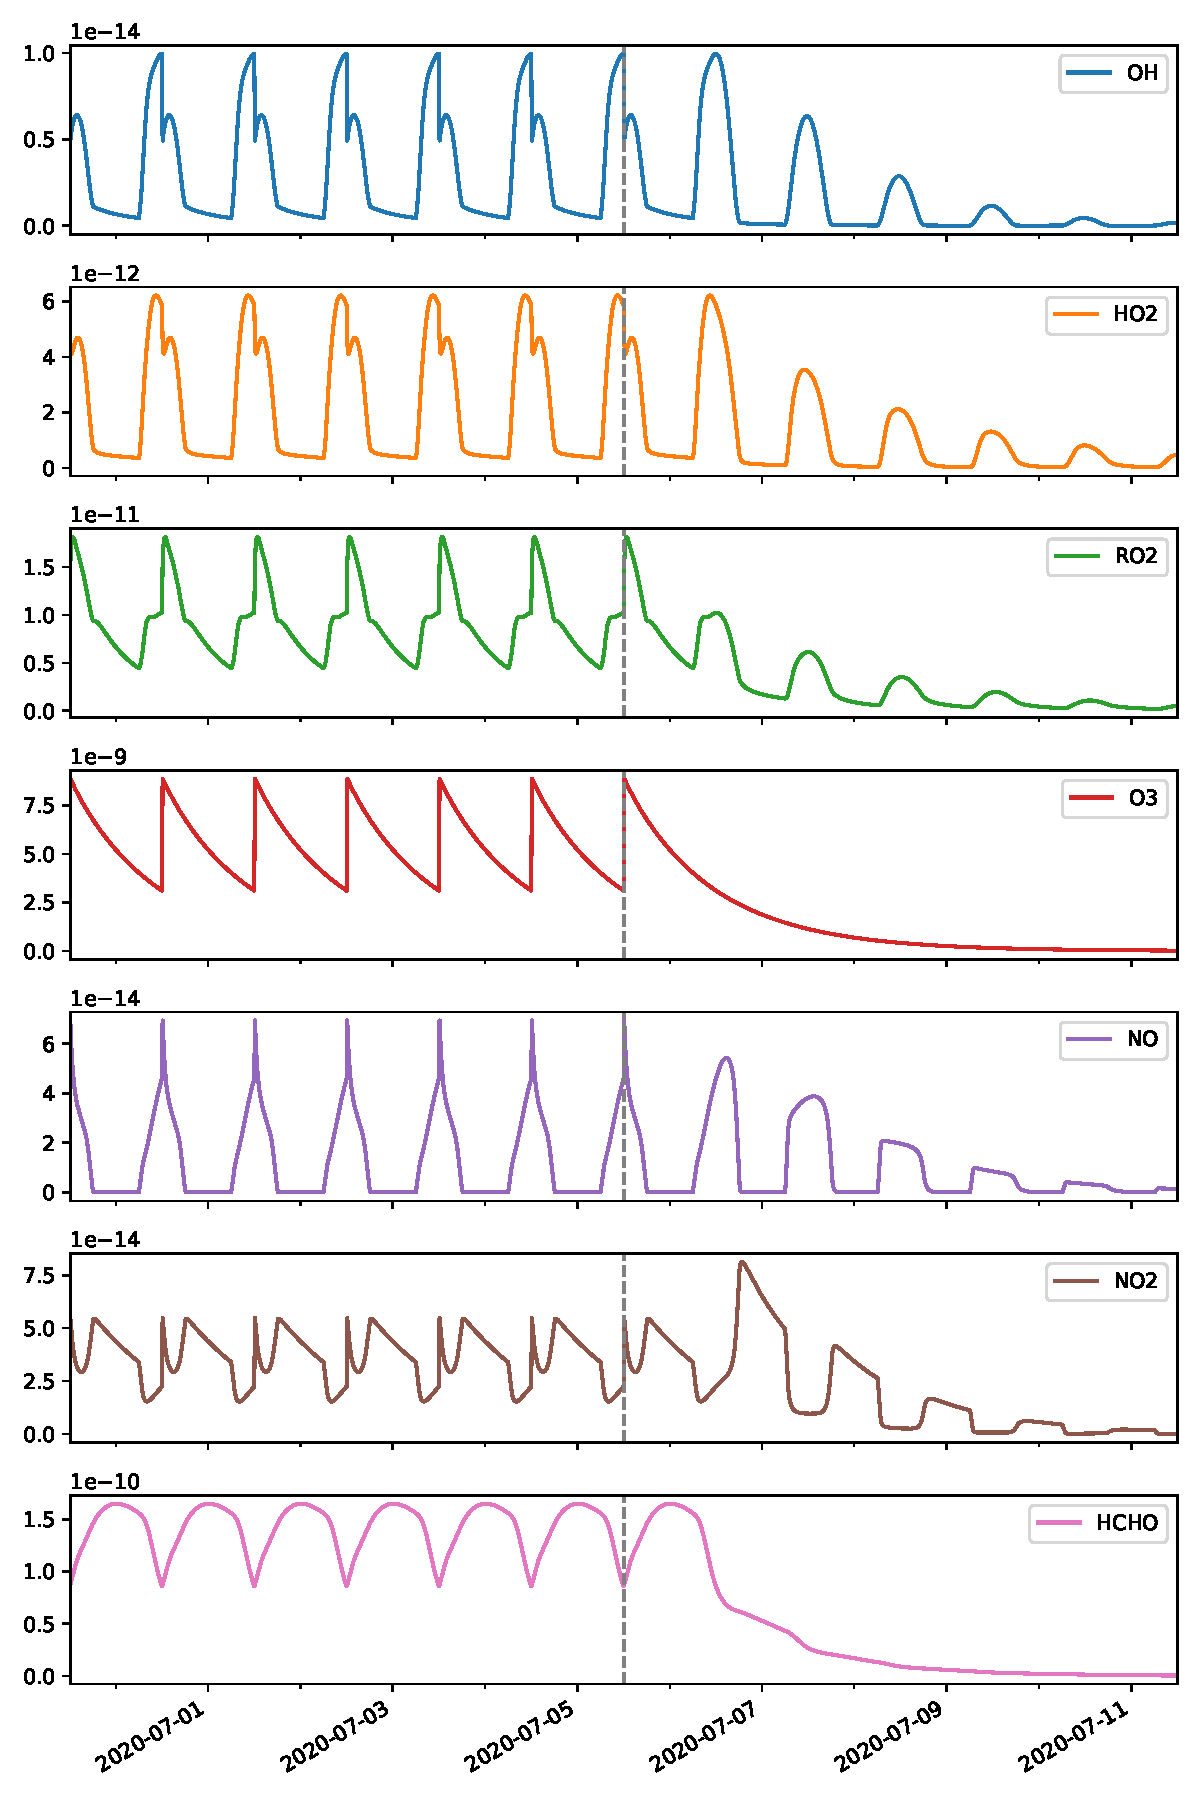
\includegraphics[width=.9\textwidth]{figures_c3/mlpregressor/conc_borneo.pdf}
\label{fig:cborneo}
\caption{\textbf{The concentration profile for Borneo.}This shows a the change in concentration over time for HO$_x$,NO$_x$,Ozone and RO$_2$ species for a simulation run generated by the mlpregressor. Left of the dashed line shows the last 6 days of spinup, where the intial concentrations are reset at noon each day until the species fractional difference is less than 0.001 .}
\end{figure}

\newpage


\begin{figure}[H]
    \centering
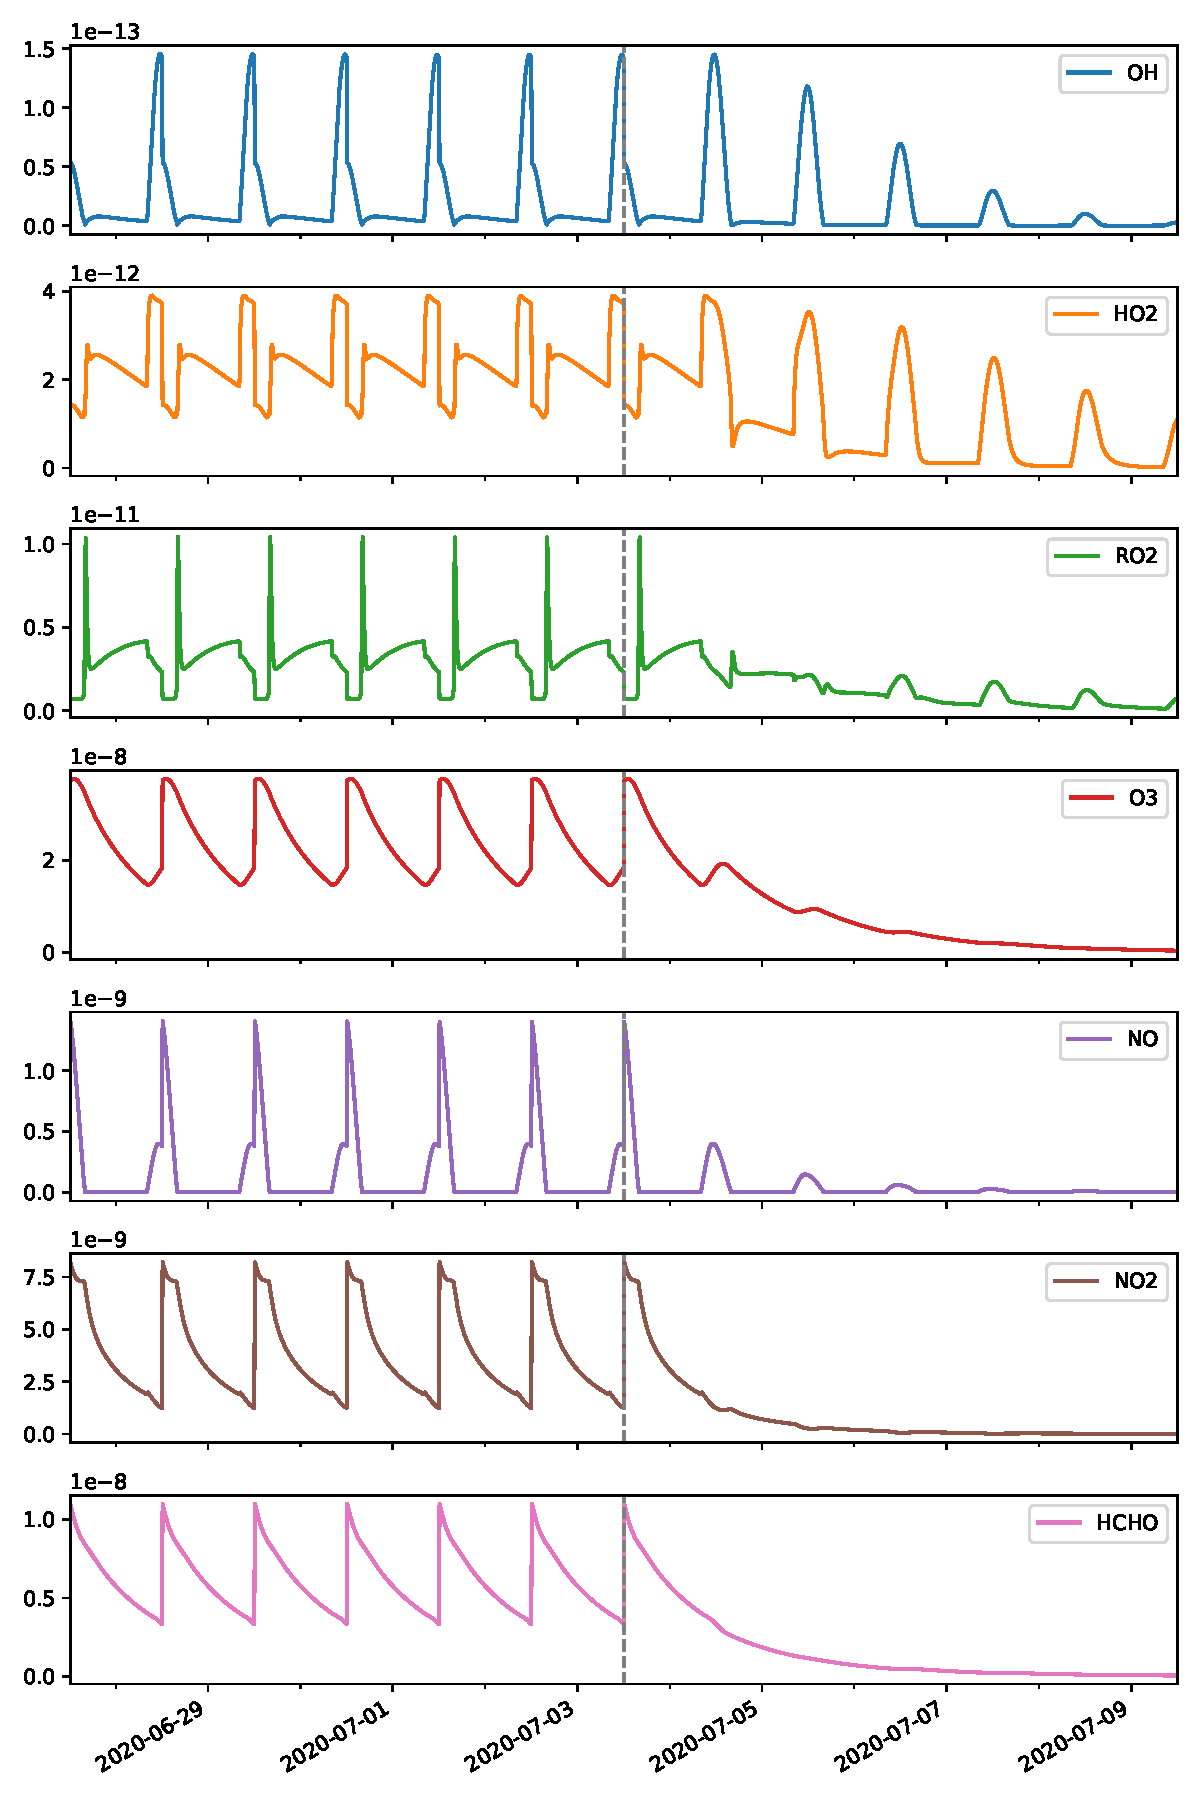
\includegraphics[width=.9\textwidth]{figures_c3/mlpregressor/conc_clfo.pdf}
\label{fig:clondon}
\caption{\textbf{The concentration profile for London.}This shows a the change in concentration over time for HO$_x$,NO$_x$,Ozone and RO$_2$ species for a simulation run generated by the mlpregressor. Left of the dashed line shows the last 6 days of spinup, where the intial concentrations are reset at noon each day until the species fractional difference is less than 0.001 .}
\end{figure}

\newpage


\begin{figure}[H]
    \centering
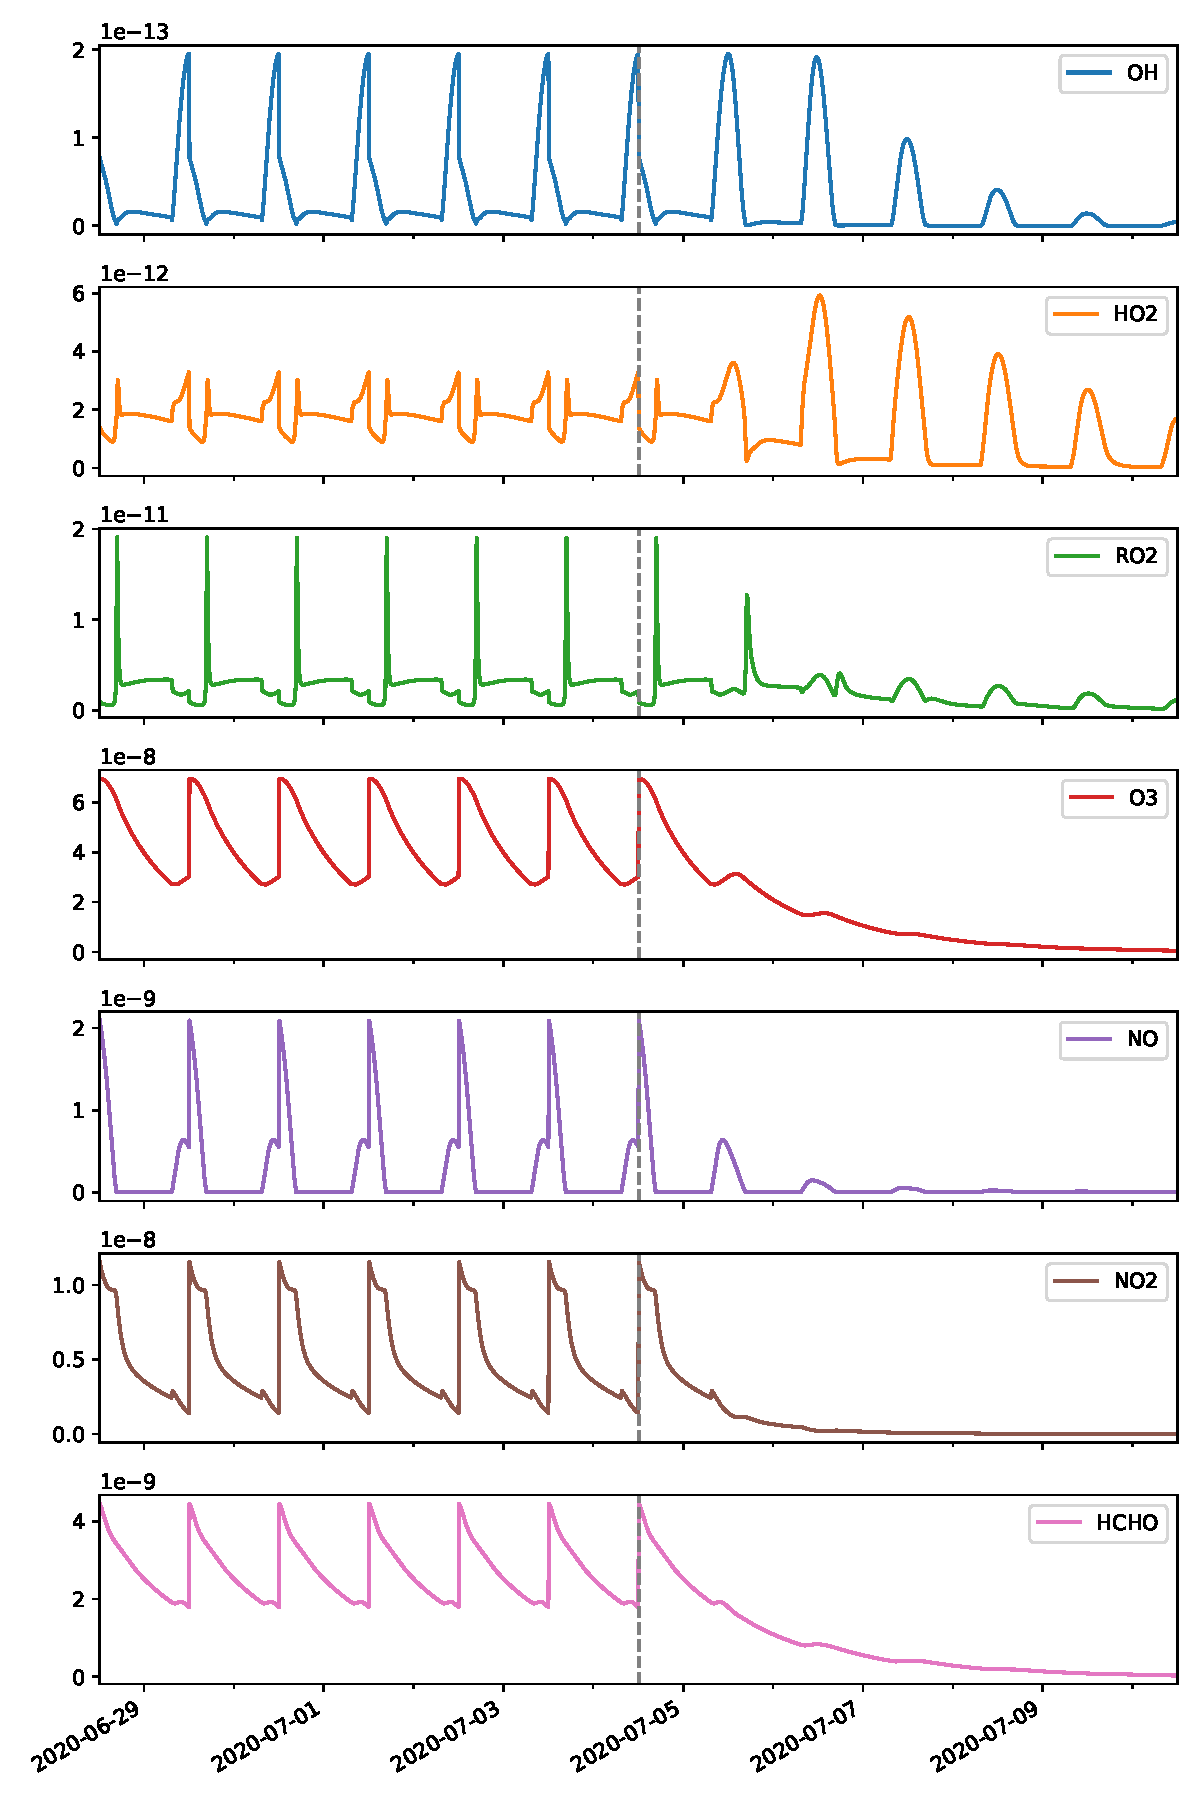
\includegraphics[width=.9\textwidth]{figures_c3/mlpregressor/conc_beijing.pdf}
\label{fig:cbeijing}
\caption{\textbf{The concentration profile for Beijing.}This shows a the change in concentration over time for HO$_x$,NO$_x$,Ozone and RO$_2$ species for a simulation run generated by the mlpregressor. Left of the dashed line shows the last 6 days of spinup, where the intial concentrations are reset at noon each day until the species fractional difference is less than 0.001 .}
\end{figure}

\newpage





\subsection{Comparing Results}
This subsection presenets the comparison between traditional model diagnostic methods and the different graph metrics. It shall also provide an inter-senario comparison between the different types of chemistry which exists in each simulation. 

Since each simulation consists of several thousand species, it is infeisable to attempt to directly compare them for each centrality metrics. This is especially true for species that may not be consistently important across all metrics. To overcome this a computational method for extracting keywords from a corpus of documents, Term Frequency - Inverse Document Frequency (TF-IDF), will be used. 

\subsubsection{The inner workings of TF-IDF}
TF-IDF is a numerical statistuc used in text natural language processing and text mining to identify the importance of a word with regard to its context. It provides a value for the frequency a word appears within a section, offset by the number of times it appears in other sections - It is for this reason that 83\% of text recommender systems in digital libraries use TF-IDF, \citep{tf83}. 

 In \citep{frankenstein} I applied this to the chapters of frankenstein, and found the keywords extracted almost exactly replicated those from the synoptic description of the novel. Although TF-IDF is a text mining procedure, the algorithm itself is mathematical, meaning that it may be applied to our diagnostic dataset. The working of the algorithm are discussed below.

\paragraph*{Term Frequency}
The TF from the algorithm name stands for term frequency. This is an analysis of the number of times a word exists within a dataset. There are several ways in which this can be done, these are:

\begin{itemize}
    \item[-] \textbf{Raw Count} - The \textit{number of times} a word exists within the document.
    \item[-] \textbf{Boolean/Logistic} - $True$ if the word exists, false otherwise.
    \item[-] \textbf{Adjusted for Document Length} -  $word\ frequency / total\ number\ of\ words$
    \item[-] \textbf{Log Scaled} - $\log(1+frequency)$
\end{itemize}

As the scaled values for each item are taken, we can liken our results to the `Adjusted for Document length' equation and use the scaled ranking value for each group respectively.

\paragraph*{Inverse Document Frequency}
Inverse document frequency tell us how much information a word provides with respect to a certain context. Whilst a word may be used extensively throughout the corpus (term frequency) we are often interested in words which ocuur often only in a single section. This is one of the reason TF-IDF is useful in the extraction of keywords from a document. 


To complete the TF-IDF equation, the term frequency and inverse document frequency terms are multiplied together. 

\begin{figure}[H]
     \centering
         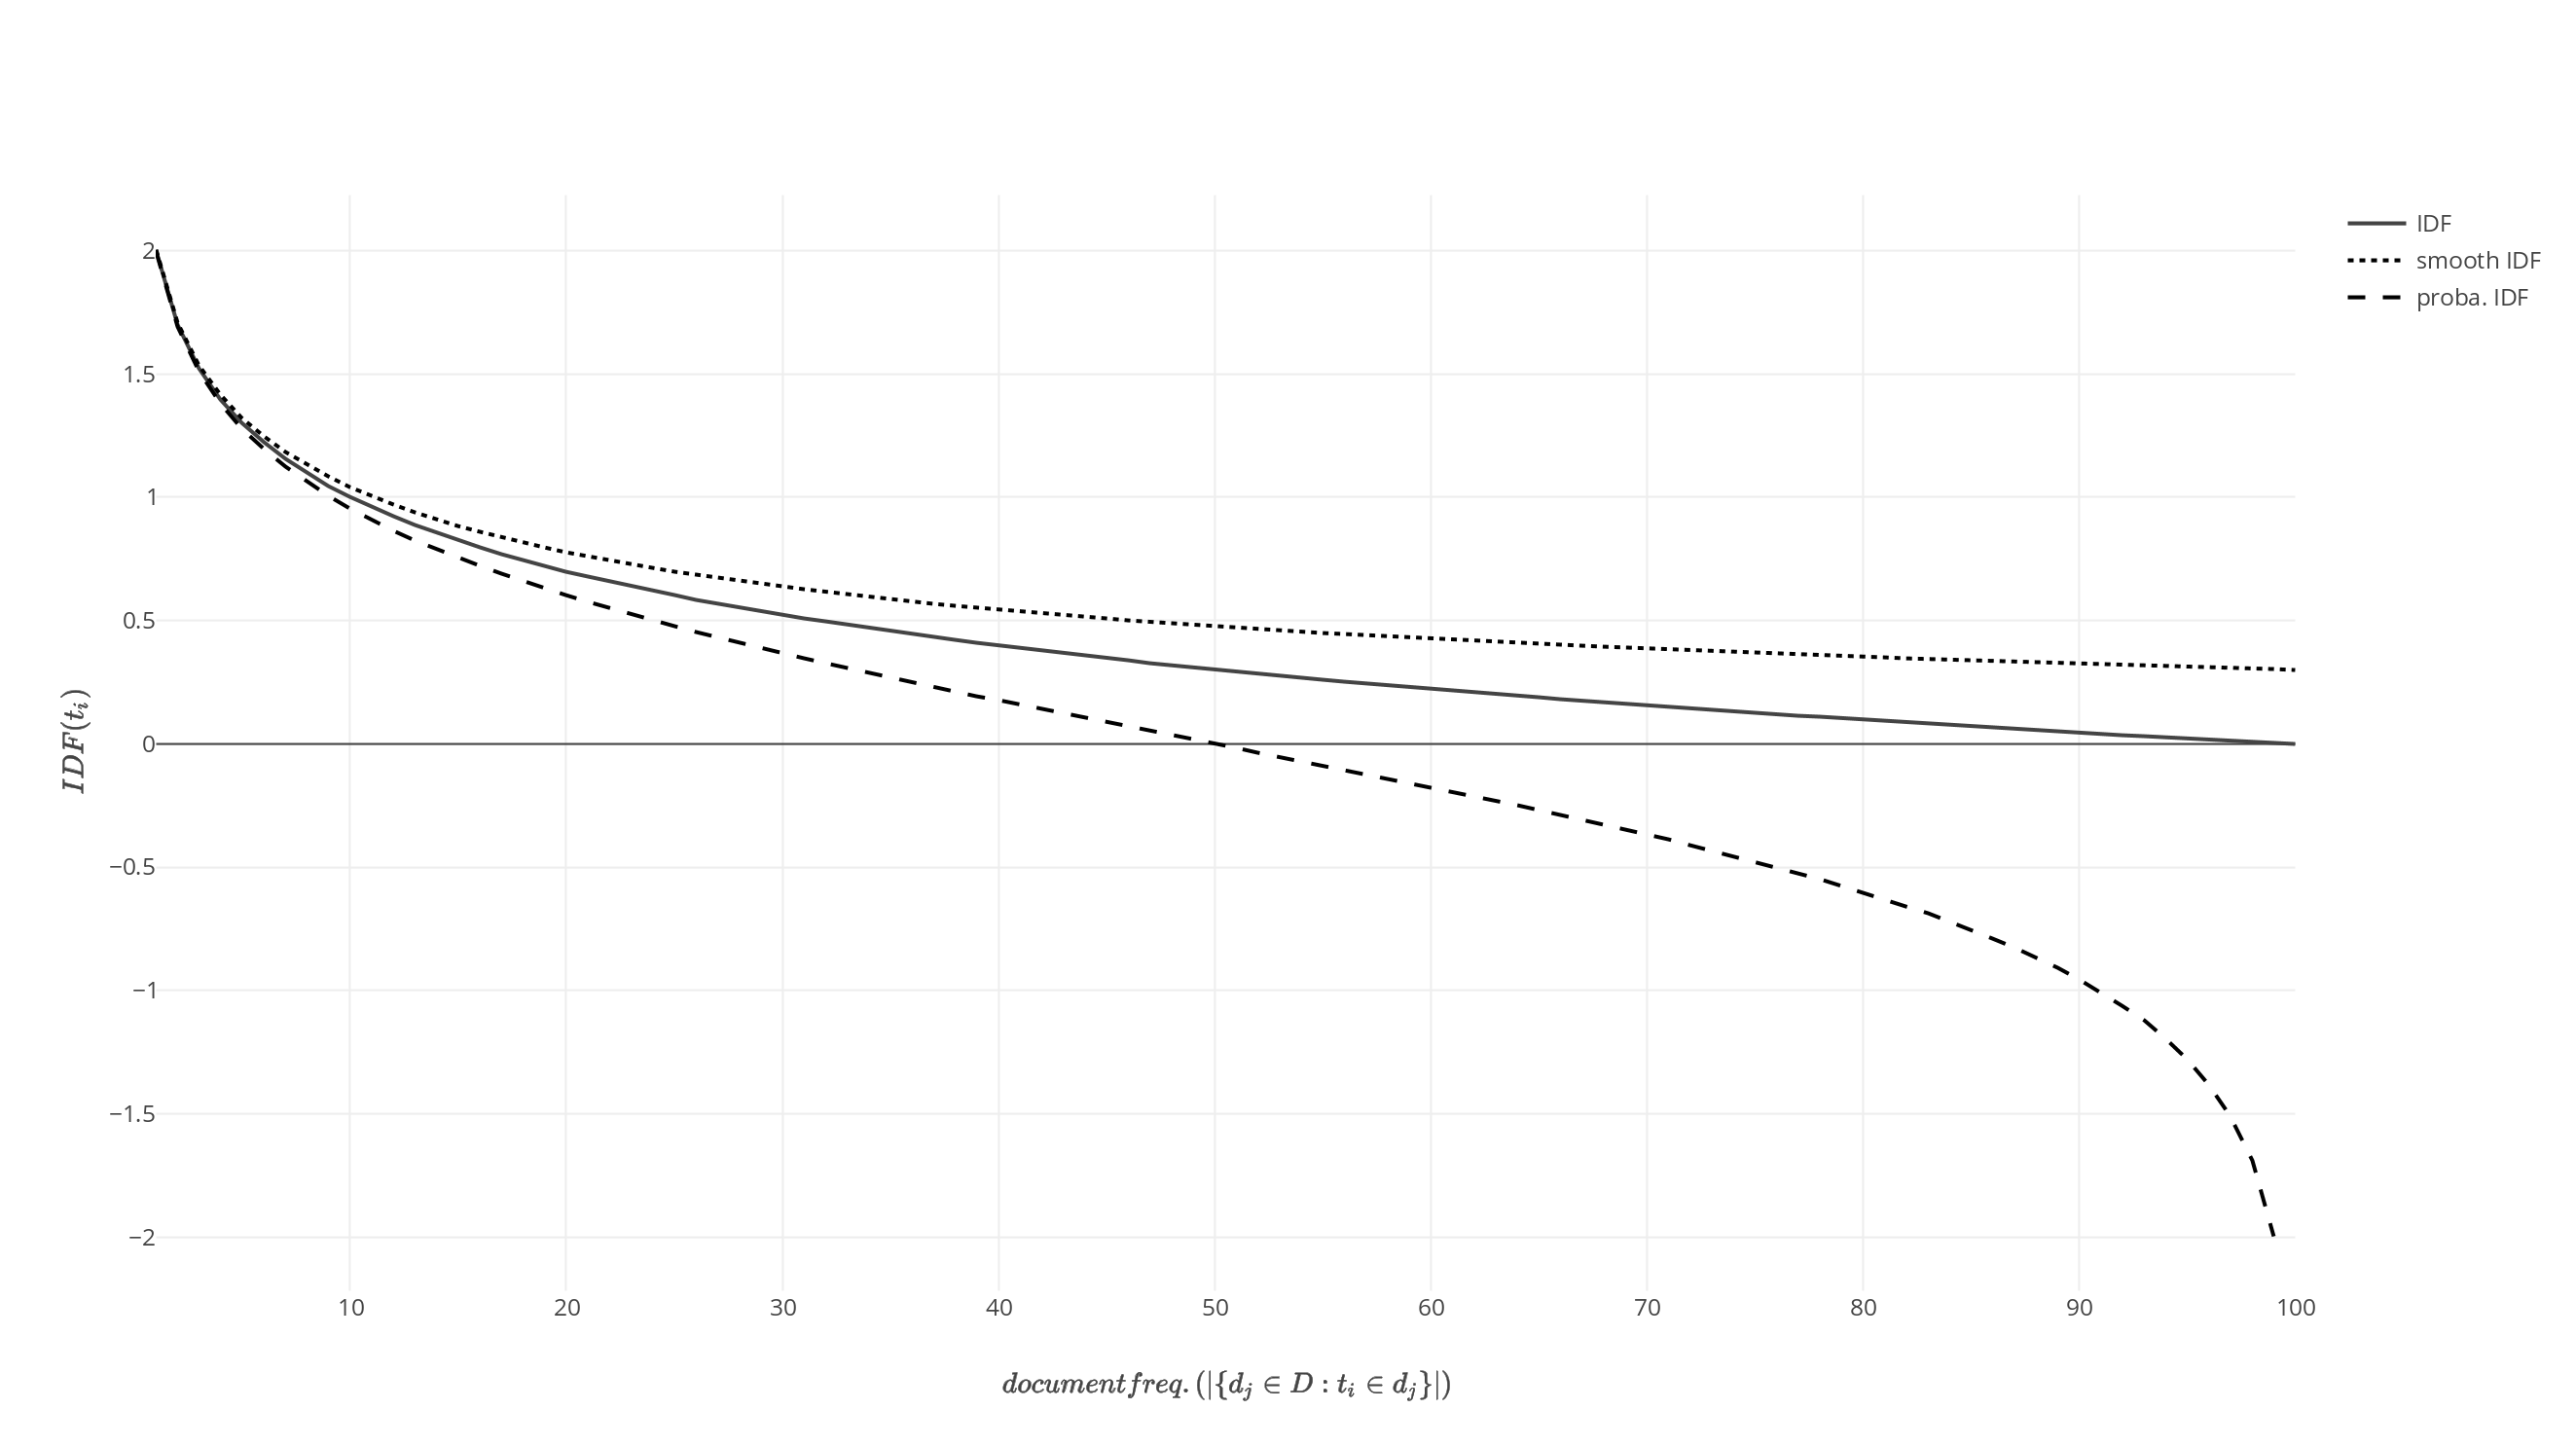
\includegraphics[width=\textwidth]{figures_c3/mlpregressor/plotidf.png}
        \caption{ \textbf{The different IDF outputs.} A plot showing Inverse Document Frequency profiles against Document Frequency. This shows that the probabalistic IDF hilights words that are more important across all items, whilst the smooth IDF shows files which are more important individually. The general IDF (which is used) produces a result starting at 2 and tending to zero. This provides the best response and can easily be scaled between the range of [0,1] by dividing the output by 2.  Source: \citep{idfpic}}
        \label{fig:idf}
\end{figure}


\paragraph*{Applying TF-IDF to chemical metrics}
As the point of interest is in identifying species which are only important to a specific metric, and not across all, it is possible to adapt the TF-IDF equation. As the Term Frequency correspoinds to the number of times a value appears within the body of a document, the scaled metric value may be used. Next this is devided by the log of the Inverse Document Frequency. The Documnent Frequency can be given as the sum of values across all metrics. This makes the TF-IDF equation: 

\begin{equation}
    TF.IDF = metric\_value\  .\ \log(\frac{N_o\ documents}{ \Sigma_\forall\ metric\_values})
\end{equation}




\subsection{Metric Comparison}

The aim of this section is to compare the efficiency of graph metrics against a list of traditional methods. To do this the use of a bivariate colourmap (\autoref{fig:cmap}) is used. Each figure consists of a red hued image/heatmap representing the scaled values \{0,1\}:\{white,red\} for each of the individual columns. As each simulation contains thousands of species, only the top 10 species from each column/category are selected. These are then sorted by the average sum of their closeness, betweenness and page-rank values (blue column). Superimposed on this reds-only heatmap is a blue heatmap representing the average sum of the three metrics for comparison. Such a method allows for the comparison of individual values against a an approximation of species importance, by the sum of graph metrics. This allows us to partition the data into different categories. 

\begin{itemize}
\item[-] \textbf{Purple} - This value is high in both the individual category and the metric sum. 
\item[-] \textbf{Red} - This value is high for the individual category but not the metric sum. 
\item[-] \textbf{Blue} - This value is high for the metric sum but not the individual category. 
\item[-] \textbf{White} - This value is low for all categories. 
\end{itemize}



\begin{figure}[H]
     \centering
         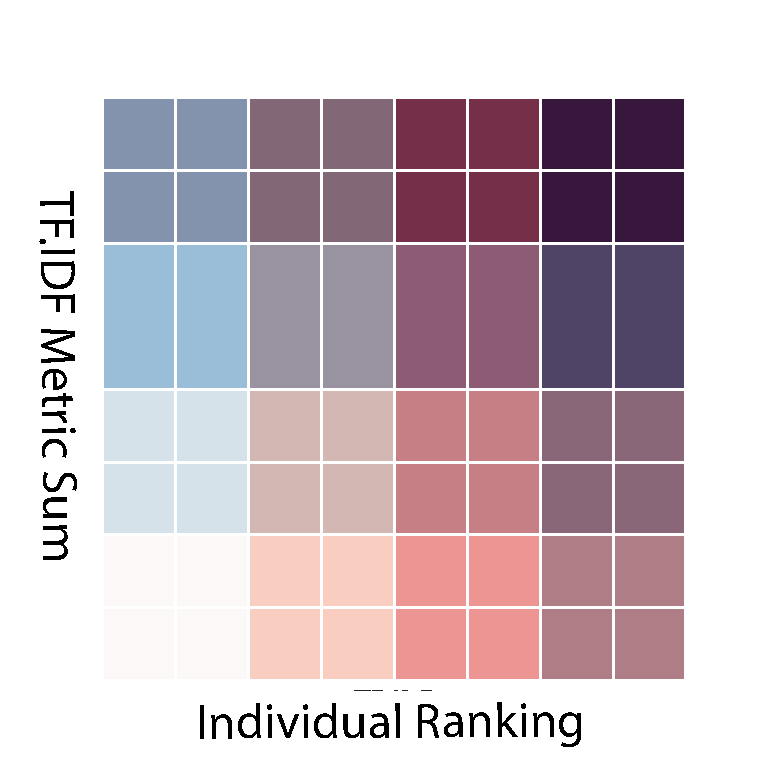
\includegraphics[width=0.4\textwidth,angle=45]{figures_c3/mlpregressor/cbar.pdf}
        \caption{ \textbf{The bivariate colourplot key.} }
        \label{fig:cmap}
\end{figure}


\subsubsection{Individual Categories}
Individual categories are split between traditional metrics and graph centrality metrics. To represent the importance of a species the following values may be extracted through the use of a simple box model:

\begin{itemize}
\item[-] \textbf{Concentration} - This describes the abundance of a species within the atmosphere. 
\item[-] \textbf{Net Flux} - This describes the rate of net (absolute) change of concentration over time for a species. 
\item[-] \textbf{Absolute Flux} - Some species may have a large flux going through them (production and loss), resulting in a small net flux. This sums the production and loss fluxes. 
\item[-] \textbf{Influence} - Influence is the total magnitude of an effect that changing a species concentration by 1\% would have on other species within the network. Since the graph is generated using the Jacobian matrix, an alternative method for calculating this can be by calculating the total out-degree of a node.  
\end{itemize}



The importance of a species is then compared through the use of three of the most common centrality metrics. These are:


\begin{itemize}
\item[-] \textbf{Centrality} - This describes how easily information from one node can be disseminated to all other nodes. 
\item[-] \textbf{Betweenness} - This describes the number of shortest paths (fastest fluxes/greatest influences) that are routed between nodes adjacent to our chosen node. Species with a high betweenness hold a brokering position, and can act as a bottleneck between different groups of chemistry. 
\item[-] \textbf{PageRank} - PageRank looks at the flow in a system. It ranks nodes not only on the number of species it reacts with, but also the importance of the species it has reacted with

\end{itemize}

Finally the `Metric Sum' is the sum of all the metric values scaled between 1 and zero (the mean).

\subsection{•}




\section{Calculating production sensetivity using personalised page rank.}

% http://sibiu.cs.vt.edu/eprints/id/eprint/282/1/Sandu_2003_KPPSEN1.pdf
% The adjoint modeling is presented as an ecient tool to evaluate the sensitivity
% of a scalar response function with respect to the initial conditions and model parameters. In addition,
% sensitivity with respect to time dependent model parameters may be obtained through a single backward
% integration of the adjoint model

\begin{figure}[H]
    \centering
\begin{subfigure}{.9\textwidth}
  \centering
  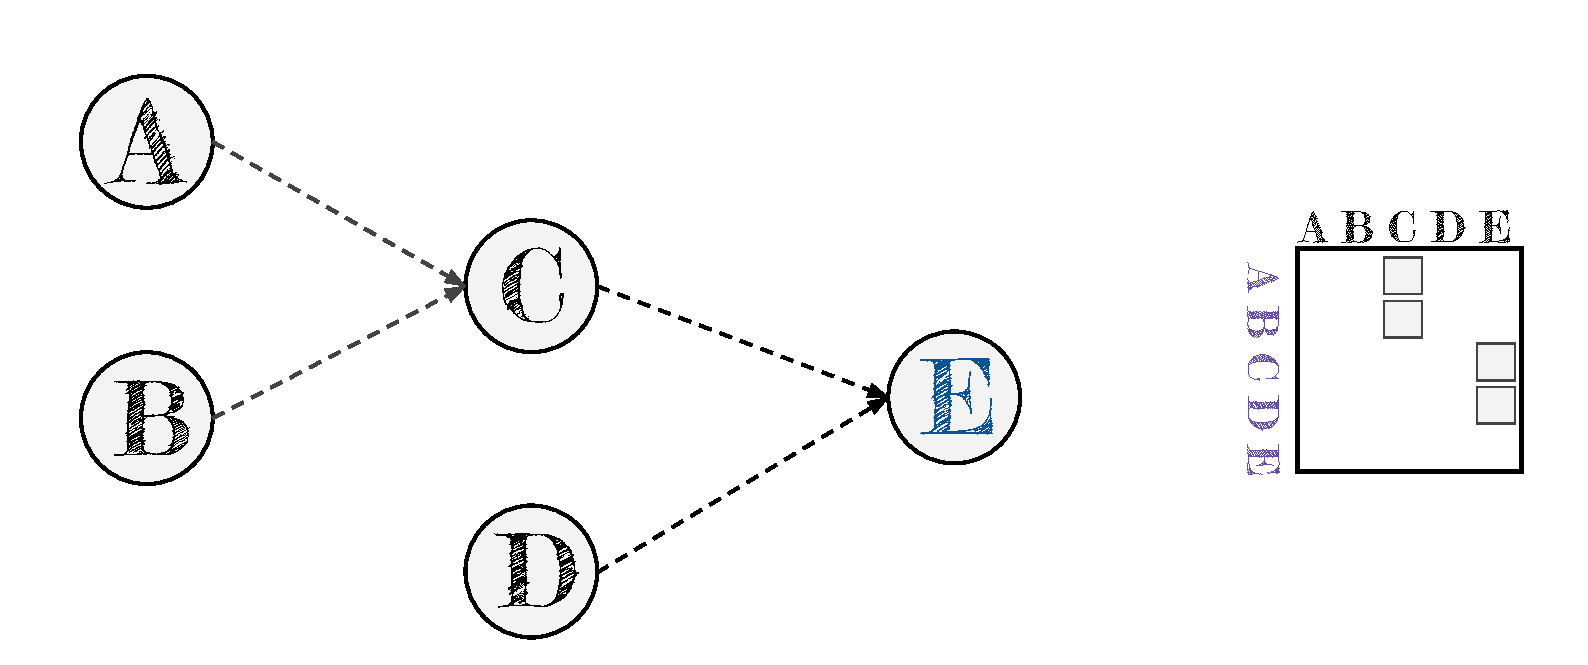
\includegraphics[width=\textwidth]{figures_c3/traditional.pdf}
  \label{fig:prtrad}
  \caption{Traditional Influence Graph}
\end{subfigure}

\begin{subfigure}{.9\textwidth }
  \centering
  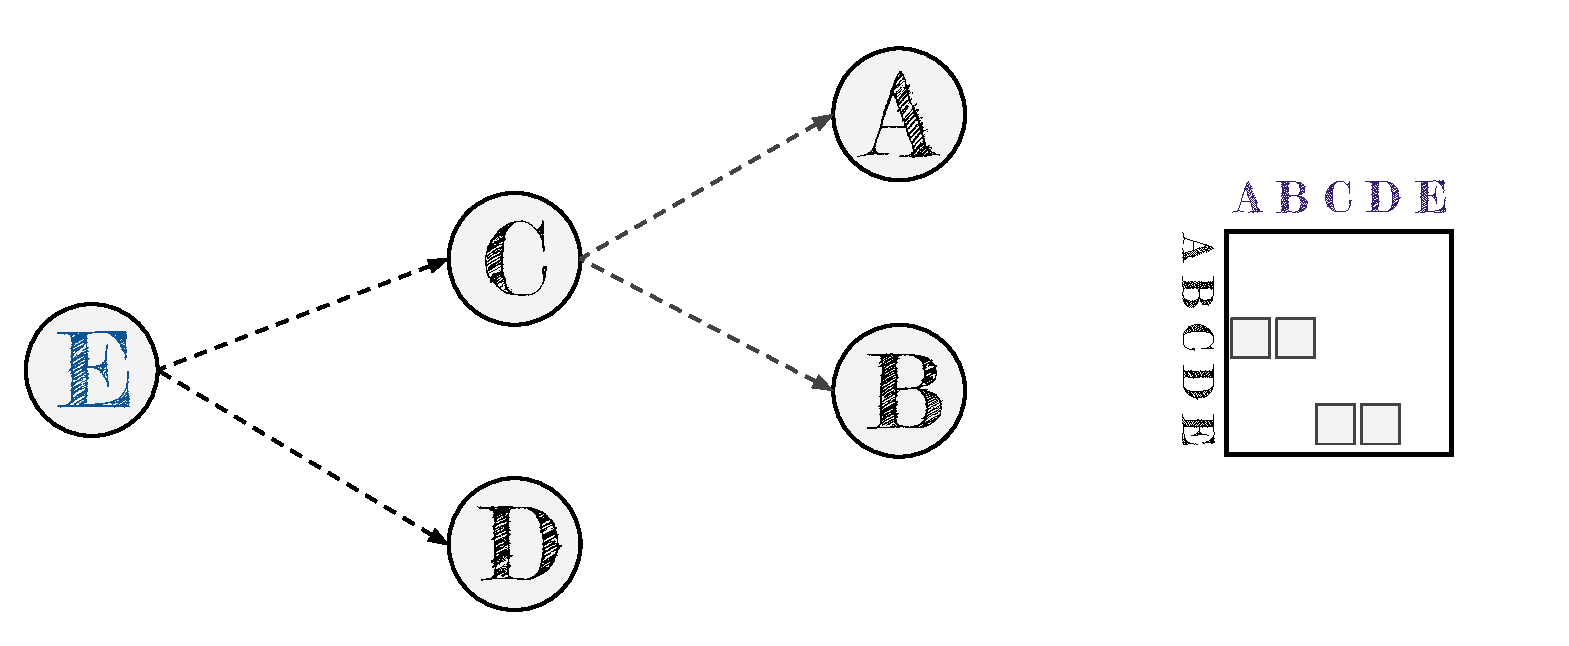
\includegraphics[width=\textwidth]{figures_c3/adjoint.pdf}
  \label{fig:pradj}
  \caption{Reversed-link (adjoint) influence graph}
\end{subfigure}

\caption{\textbf{Link reversal of the Jacobian Sensetivity matrix graph results in a graph of the Adjoint.} Showing how in changing the direction of the links in a graph is equivalent to applying the transpose to an adjacency matrix (right). In the case of a Jacobian based graph, this is analogous to using the adjoint to propagate the model back in time - something that can be used to identify the influence upon a species with a model.}
\end{figure}


\subsection{Testing}
Borneo


As with all scintific processes, it is importatnt to first test the algorithm on a small, comprehensible example. To do this we start with the creation of \ch{ch2oo}. This is a direct product of isoprene. In tracing back all the precursors the mechanism for its creation can be described as: 

\begin{equation}
    \ce{O3 + C5H8 ->[\kappa] CH2OOE}+(MACR\ or\ MVK)\\
    \ce{CH2OOE -> [\kappa_{dec}] CH2OO}
\end{equation}

In traversing the adjoint/reversed graph, this presenets a singe `shortest path' between the product and its precursor. This creates for a base test for the algorithm. The PageRank algorithm is now run with a personalisation vector consisting with an value of 1000000 for the species of interest and -1 for all others. A damping factor value of 0.01 is also used for the algorithm. 

As \ce{CH2OOE} only has one precursor ($\alpha$-pinene) the initial test is done on this. From this the identification of isoprene as a source is sucessful, although since the algorithm is performed on the whole network, there are results for a number of additional species, \autoref{tab:ch2ooe}. This is because page rank works on using teleporation to change between items in the evolution of the system. With the design of the personalisation vector, these values will however be significantly smaller than any containing useful results. 


\begin{table}[H]
    \begin{tabular}{lr}
\toprule
{} &             1 \\
0       &               \\
\midrule
\ch{C5H8}    &  9.920000e-03 \\
\ch{CH2OOE}  &  9.920000e-01 \\
\ch{C816O}   & -9.990000e-07 \\
\ch{NC101CO} & -9.990000e-07 \\
\ch{C926OH}  & -9.990000e-07 \\
\bottomrule
\end{tabular}
\label{tab:ch2ooe}
\caption{A reversed graph Page Rank test with \ce{C5H8 + O3 -> CH2OOE} as the only reaction.}
\end{table} 

Next we apply the same methodology to \ce{CH2OO}. This creates the graph in \autoref{fig:prtest0}. Here it is seen that \ce{CH2OO} is directly dependant on the radicals \ce{CH2OO[F,B,C,G,A]}, and \ce{CH2OOE}. This is then dependant on Isoprene, which then has a range of dependancies with all have precursors of their own (not shown). 


\begin{figure}[H]
  \centering
  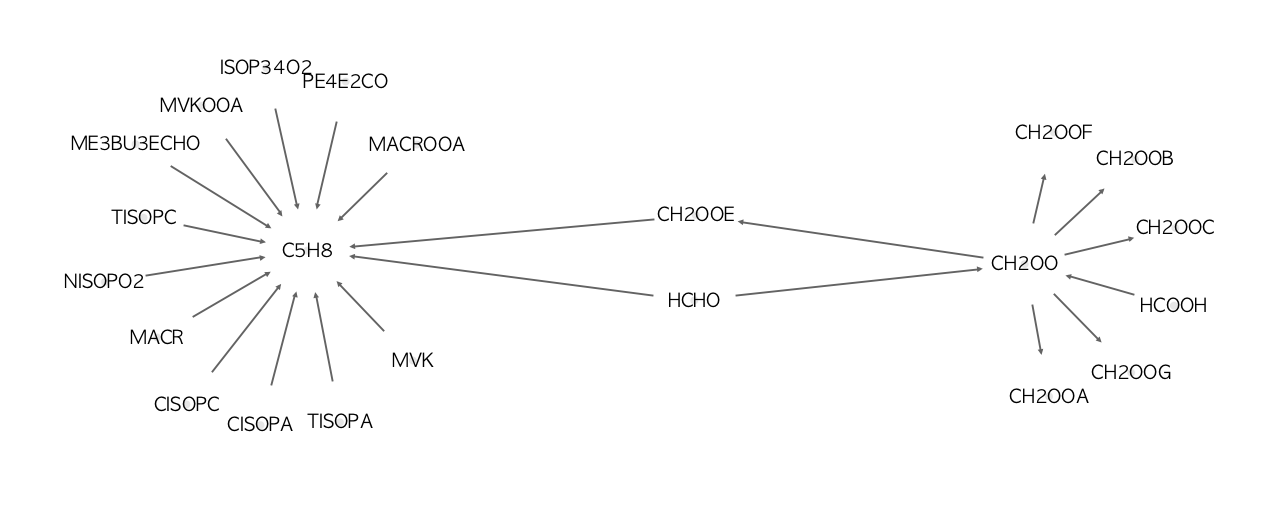
\includegraphics[width=\textwidth]{figures_c3/prtest0.png}

  \label{fig:prtest0}

\caption{\textbf{The reversed subgraph between Isoprene, \ce{CH2OOE} and \ce{CH2OO}.} This is a subgraph of the afforementioned species, showing them and their neighbours. Here the arrows point towards a species precursor. }
\end{figure}

\begin{table}[H]
    \begin{tabular}{lr}
    \toprule
    {} &         1 \\
    0          &           \\
    \midrule
    CH2OO      &  0.992000 \\
    CH2OOE     &  0.001670 \\
    CH2OOF     &  0.001660 \\
    CH2OOG     &  0.001660 \\
    CH2OOA     &  0.001660 \\
    CH2OOC     &  0.001640 \\
    CH2OOB     &  0.001640 \\
    C5H8       &  0.000016 \\
    MACR       &  0.000016 \\
    C2H4       &  0.000007 \\
    HMACR      &  0.000007 \\
    ISOP34NO3  &  0.000005 \\
    ME3BU3ECHO &  0.000005 \\
    ISOPDNO3   &  0.000004 \\
    C622CHO    &  0.000002 \\
    C624CHO    &  0.000002 \\
    C518CHO    &  0.000002 \\
    C729CHO    &  0.000002 \\
    LIMAL      &  0.000002 \\
    C3H6       &  0.000001 \\
    BUT1ENE    &  0.000001 \\
    PE4E2CO    &  0.000001 \\
    MVK        &  0.000001 \\
    MVKOH      &  0.000001 \\
    ISOPBNO3   &  0.000001 \\
    ACR        &  0.000001 \\
    \bottomrule
    \end{tabular}
\label{tab:ch2ooe}
\caption{A reversed graph Page Rank test with \ce{C5H8 + O3 -> CH2OOE} as the only reaction.}
\end{table} 

